\documentclass[a4paper,12pt]{article}
\usepackage{array}
\usepackage{enumitem}
\usepackage[a4paper]{geometry}
\usepackage[english,italian]{babel}
\usepackage{amsmath}
\usepackage{dsfont}
\usepackage{graphicx}
\usepackage{hyperref}
\usepackage{url}
\usepackage[utf8]{inputenc}
\usepackage{bookmark}

\geometry{left=33mm, right=30mm}

\title{
	IoTeX
	\linebreak
	\Large Una Rete Decentralizzata per l'Internet of Things
	\linebreak
	\Large Basata su una Blockchain Incentrata sulla Privacy}
	\author{Il Team IoTeX (support@iotex.io)}
	\date{Ultimo Aggiornamento: 12 Luglio, 2018
	\linebreak Version 1.5
	}


\begin{document}

\maketitle

\vspace{200pt}


\textbf{Dichiarazione di limitazione di responsabilità.} Questo documento deve essere inteso come una panoramica tecnica. Non vuole essere esaustivo, né rappresentare un progetto definitivo; pertanto aspetti secondari, come API, interconnessioni o linguaggi di programmazione, non vengono trattati.

\pagebreak

\begin{abstract}
	La maggior parte dei dispositivi IoT (Internet of Things), sebbene decentralizzati per natura, ad oggi vengono distribuiti in modo centralizzato. Molti problemi sono emersi: scalabilità, costi operativi elevati, problemi di privacy, rischi per la sicurezza, e mancanza di valore funzionale. La Blockchain, decentralizzata per definizione, può rappresentare una buona soluzione a questi problemi. Innanzitutto, la blockchain è abbastanza elastica da risolvere la sfida della scalabilità dell'IoT in modo economicamente vantaggioso. In secondo luogo, mantenendo i dati all'interno di blockchain ben definite, si eliminano i timori per i dati IoT memorizzati in cloud, potenzialmente suscettibili di trapelare o di essere violati. In terzo luogo, le blockchain con smart contract e token hanno un enorme potenziale per consentire il coordinamento autonomo dei dispositivi al fine di creare valore funzionale. Tuttavia, le blockchain esistenti hanno i loro limiti nell'affrontare i problemi dell'IoT, a causa delle caratteristiche peculiari che lo contraddistinguono, ad esempio la grande quantità e l'eterogeneità dei dispositivi, i limiti nella potenza di elaborazione, nell'archiviazione dati, nell'alimentazione, ecc.
	Questo documento introduce IoTeX, una rete decentralizzata per l'IoT basata su una blockchain incentrata sulla privacy, con quattro importanti innovazioni:

	\begin{itemize}

		\item
		      Blockchain in blockchain, per una rete distribuita ben bilanciata che massimizza la scalabilità e la privacy in modo economicamente vantaggioso;

		\item
		      Privacy reale integrata sulla blockchain, basata sui meccanismi di \emph{codice di pagamento inoltrabile}, \emph{ring signature a dimensione costante} e senza configurazione \emph{trusted}, e una implementazione iniziale del \emph{Bulletproof};

		\item
		      Consenso rapido con finalità immediata, per migliorare notevolmente l'efficienza della rete, e ridurre i costi di transazione;

		\item
		      Architetture flessibili e leggere, per la realizzazione delle applicazioni IoT chiave in molteplici settori industriali.

	\end{itemize}

\end{abstract}

\pagebreak

\tableofcontents

\pagebreak

\section{L'Internet of Things}
L'Internet of Things (IoT) sta emergendo rapidamente come manifestazione della visione di una società collegata in rete: qualsiasi cosa che beneficia di una connessione, è connesso. Eppure, questa trasformazione su vasta scala rappresenta solo l'inizio. Il numero di dispositivi IoT è destinato a crescere del 21\% ogni anno, raggiungendo i 18 miliardi nel 2022 \cite{c10}, mentre il mercato globale dell'IoT è destinato a passare dai 170 miliardi di dollari del 2017 a 560 miliardi di dollari entro il 2022 \cite{c15}, con un tasso di crescita annua del 26,9\%. Sebbene molti esperti dell'industria e consumatori entusiasti hanno definito l'IoT come la prossima rivoluzione industriale o il prossimo internet, ci sono tre problemi principali che frenano in maniera massiccia lo sviluppo e l'adozione dell'IoT.

\subsection{Il problema della scalabilità}
La maggior parte dei dispositivi IoT sono ad oggi connessi e controllati in maniera centralizzata. I dispositivi IoT sono connessi ad infrastrutture di back-end, su servizi cloud pubblici oppure localmente all'interno di server farm, per trasmettere dati oppure ricevere comandi di controllo.
Attualmente, la dimensione dell IoT è strozzata dal livello di scalabilità ed elasticità di queste infrastrutture di back-end, server e data center. E' improbabile che il costo operativo sostanzialmente elevato necessario per scalare l'IoT sia coperto dai profitti della vendita dei dispositivi. Di conseguenza, molti fornitori IoT non riescono a proporre dispositivi economicamente vantaggiosi ed applicazioni che siano abbastanza scalabili ed affidabili per scenari reali.

\subsection{Mancanza di Privacy}
Si prevede che l'IoT permetterà la partecipazione di massa degli utenti finali a servizi mission critical come l'energia, la  mobilità, la stabilità legale e democratica. Le sfide per la privacy hanno origine dal fatto che l'IoT interagisce con il mondo fisico in modi diretti e automatici, e la quantità di dati raccolti aumenterà notevolmente quando si ridimensionerà. Alcune  delle minacce alla privacy comuni, come elencate in \cite{c37}, sono:

\begin{enumerate}

	\item
	      Identificazione: associare un identificatore  persistente), ad es. Un nome e un indirizzo o uno pseudonimo di qualsiasi tipo, con un individuo;
	\item
	      Localizzazione e tracciamento: ottenere la posizione di un individuo attraverso diversi mezzi;
	\item
	      Profilazione: Compilare fascicoli informativi sulle persone per dedurrne gli interessi per
	      associazione con altri profili e fonti di dati;
	\item
	      Interazione e presentazione che violano la privacy: trasmettere informazioni private attraverso un mezzo pubblico e nel processo rivelarle ad un pubblico indesiderato;
	\item
	      Transizioni del ciclo di vita: i dispositivi spesso memorizzano enormi quantità di dati sulla propria storia durante l'intero ciclo di vita che potrebbe trapelare durante i cambiamenti della sfera di controllo nel ciclo di vita di un dispositivo;
	\item
	      Attacco all'inventario: raccolta non autorizzata di informazioni sull'esistenza e sulle caratteristiche degli oggetti personali, ad esempio, i ladri d'appartamento potrebbero utilizzare l'inventario dati per controllare la proprietà, e individuare un momento sicuro per entrare;
	\item
	      Collegamento: collegamento di sistemi diversi precedentemente separati in modo tale che la combinazione delle fonti di dati riveli informazioni (vere o errate) che il soggetto non aveva rivelato alle fonti isolate e, soprattutto, che non intendeva rivelare.
\end{enumerate}
Tutte queste tipiche minacce alla privacy sono dovute a perdite di dati a livello del dispositivo, oppure alla perdita di dati durante la comunicazione, o più spesso alla perdita di dati nella parte centralizzata della rete.

\subsection{Mancanza di Valore Funzionale}
La maggior parte delle soluzioni IoT esistenti non crea valore significativo. Il solo "Essere connesso" rappresenta la proposta di valore più utilizzata. Tuttavia, abilitare semplicemente la connettività non rende un dispositivo intelligente o utile. La maggior parte del valore che l'IoT produce è dovuto all'interazione, alla cooperazione, ed infine dal coordinamento autonomo di entità eterogenee. Alcune buone analogie sono le singole cellule che cooperano per costruire gli organismi multicellulari, gli insetti che insieme costruiscono società, oppure gli uomini che costituiscono città e stati. Grazie alla cooperazione, tutti questi individui si uniscono per costruire qualcosa che ha un valore maggiore rispetto a tutti loro isolatamente. Sfortunatamente, secondo \cite{c29}, l'85\% dei dispositivi obsoleti non hanno la capacità di interagire o cooperare tra loro, a causa di problemi di compatibilità. La condivisione dei dati per il business e le indizazioni operative è quasi impossibile.

\section{Blockchain}
La tecnologia della Blockchain è stata introdotta nel 2008 e la sua prima implementazione, ovvero Bitcoin, è stata introdotta un anno dopo, nel 2009, pubblicata nel documento \emph{Bitcoin: A Peer-to-Peer Electronic Cash System} \cite{c21} di Satoshi Nakamoto (pseudonimo). Essenzialmente, la blockchain è un database transazionale distribuito, condiviso tra tutti i nodi partecipanti nella rete. Questa è la principale innovazione tecnica di Bitcoin, ed agisce come un registro pubblico per le transazioni. Ogni nodo nel sistema ha una copia completa dello stato attuale della blockchain, che contiene ogni transazione che sia mai stata eseguita. Ogni blocco della blockchain contiene l'hash del blocco precedente, il che collega i due blocchi insieme. Tutti i nodi collegati tra loro diventano una blockchain.

\subsection{Ingredienti}
Una blockchain può essere percepita come un continuum tetra-dimensionale avente tre livelli orizzontali composti da transazioni e blocchi, consenso, e interfaccia di calcolo; e l'unico livello verticale di amministrazione (\emph{governance}).

\subsubsection{Transazioni e blocchi}
Trovandosi al livello orizzontale più in basso, le transazioni firmate vengono trasmesse tra tutti i nodi, mentre i blocchi vengono generati solo dai nodi completi (\emph{full nodes}). Questa è la base della blockchain, dove il trasferimento di beni digitali (e dunque il valore a loro associato) e la sicurezza degli account si ottengono attraverso primitive come la firma a curva ellittica, la funzione hash e il Merkle tree.

\subsubsection{Consenso}
Il livello orizzontale intermedio mostra la natura peer-to-peer della blockchain, dove tutti i nodi all'interno della rete raggiungono il consenso su tutti gli stati interni della catena attraverso tecniche come Proof of Work (PoW), Proof of Stake (PoS) e le loro varianti; Byzantine fault tolerance (BFT) e le sue varianti, \emph{etc}. Il livello di consenso interessa principalmente la scalabilità. Il PoW viene tipicamente considerato meno scalabile rispetto al PoS. Inoltre, questo livello ha un forte impatto sulla sicurezza in termini di doppia spesa ed altri attacchi che si concentrano sul modificare gli stati della blockchain in modi inattesi.

\subsubsection{Interfaccia di calcolo}
I primi due livelli orizzontali realizzano \emph{la forma} di una blockchain, mentre il livello di interfaccia di calcolo è fondamentale per garantire l'\emph{utilità} di una blockchain, il che comprende l'estendibilità ed l'usabilità. Ad esempio, Ethereum ha implementato gli smart contract per consentire la programmabilità, in modo da poter disporre di un \emph{"computer globale"} distribuito per l'esecuzione dei termini di un contratto. Anche il sidechain, insieme con il mining congiunto, sono stati sviluppati in modo intensivo per supportare la programmabilità. All'interno di protocolli di secondo livello come la rete Raiden \cite{c25}, è stato sviluppato il canale di stato per estendere la scalabilità della blockchain. Inoltre, anche gli strumenti, gli SDK, i framework e le interfacce grafiche sono estremamente importanti per l'usabilità. Il livello di interfaccia di calcolo offre agli sviluppatori la possibilità di sviluppare app decentralizzate (DApps), una funzionalità essenziale per rendere la blockchain utile e di valore.

\subsubsection{Amministrazione}
Come accade per gli organismi viventi, le blockchain di maggior successo saranno quelle che in futuro riusciranno ad adattarsi meglio al loro ambiente. Supponendo che questi sistemi debbano evolversi per sopravvivere, il progetto iniziale è importante ma, nel lungo termine, i meccanismi per il cambiamento lo saranno di più: essi sono noti come il livello verticale di amministrazione (\emph{governance}). Ci sono due componenti critici della governance:
\begin{itemize}
	\item
	      Incentivo: ogni gruppo nel sistema ha i propri incentivi. Gli incentivi non sono sempre allineati al 100\% con quelli di tutti gli altri gruppi nel sistema. I gruppi proporranno nel tempo cambiamenti che sono vantaggiosi per loro. Gli organismi sono "di parte" quando si tratta della propria sopravvivenza. Ciò normalmente si manifesta in cambiamenti nella struttura retributiva, nella politica monetaria o negli equilibri di potere.

	\item
	      Coordinamento: poiché è improbabile che tutti i gruppi risultino completamente allineati sugli incentivi in ogni momento, la capacità di ciascun gruppo di coordinarsi attorno agli incentivi comuni è fondamentale per loro per produrre un cambiamento. Se un gruppo riesce a coordinarsi meglio di un altro, crea uno squilibrio di potere a proprio favore. In pratica, un fattore decisivo per la sopravvivenza di una blockchain è quanto coordinamento si può realizzare utilizzando la blockchain (ad es. votando le regole del sistema come in Tezos \cite{c34}, o addirittura ripristinando uno stato precedente della blockchain se gli azionisti di maggioranza non gradiscono una modifica), rispetto al coordinamento che deve essere realizzato fuori dalla blockchain (come ad es. i Bitcoin Improvement Proposals (BIPs)
	      \cite{c3}).

\end{itemize}

\subsection{Modelli Operazionali}
Le blockchain possono essere categorizzate come "non autorizzate" ed "autorizzate", a seconda di come sono gestite. Ad esempio, Bitcoin è priva di autorizzazione, il che significa che chiunque può creare un indirizzo e iniziare a interagire con la rete: in questo caso si parla di "costruire fiducia in mancanza di affidabilità". Al contrario, la blockchain autorizzata è un ecosistema chiuso e monitorato, dove l'accesso di ciascun partecipante è defnito, e differenziato in base al suo ruolo: in questi casi si parla di "costruire fiducia in bassa affidabilità".
Vi sono vantaggi e svantaggi in ciascun approccio. Ad ogni modo, tutte queste considerazioni si riducono a compromessi di progetto fondamentali tra fiducia, scalabilità, elaborazione e complessità. Ad esempio, Bitcoin ed Ethereum sono blockchain costruite su nodi non affidabili, perché la scalabilità è fortemente desiderata. Quindi, o è richiesta molta elaborazione (nel caso del PoW), oppure è necessario un meccanismo di consenso più sofisticato. Al contrario, Fabric \cite{c14} è una blockchain autorizzata in cui tutti i nodi sono considerati affidabili e hanno identità crittografiche, ad esempio, rilasciate grazie ai servizi di membri come il Public Key Infrastructure (PKI), il che li rende altamente scalabili con poca elaborazione e un meccanismo di consenso relativamente semplice.

\begin{table}[htp]%
	\caption{Proprietà delle Blockchain: Benefici per l'IoT}
	\label{table:BlockchainBenefits}\centering %
	\begin{tabular}{l|l}
		\hline
		Proprietà della Blockchain  & Benefici per l'IoT       \\
		\hline
		Decentralizzazione          & Stabilità, Privacy       \\
		Bizantine Fault Tolerance   & Disponibilità, Sicurezza \\
		Trasaprenza \& Immutabilità & Assicurazione di Fiduca  \\
		Programmabilità             & Estendibilità            \\
		\hline
	\end{tabular}
\end{table}


\section{Benefici e Sfide di Blockchain e IoT}
Sensazione e percezione, trasformazione, trasmissione ed elaborazione sono l'essenza delle entità più intelligenti su questo pianeta. Per l'IoT, mentre il livello di sensazione e percezione è distribuito per definizione, gli ultimi due al momento non lo sono, e questa è la fonte della maggior parte dei problemi di scalabilità, privacy ed estensibilità. Utilizzando la blockchain come spina dorsale e sistema nervoso dell'IoT, possiamo immaginare questa tecnologia come il miglior candidato per affrontare i problemi specifici di questo mondo precedentemente menzionati.

\subsection{Benefici}
Abbracciando la tecnologia blockchain, l'IoT beneficia immediatamente dei seguenti aspetti, grazie alle proprietà intrinseche della blockchain: la decentralizzaizione, il Byzantine Fault Tolerance, la trasparenza e l'immutabilità. La Tabella \ref{table:BlockchainBenefits} riassume quali benefici queste proprietà hanno per l'IoT.


\subsubsection{Decentralizzazione}
La decentralizzazione libera gli utenti e i dispositivi dal monitoraggio esteso e controllato in modo centralizzato, dunque affrontando in parte i timori riguardanti la vita privata imposte dalle entità centralizzate che monopolizzano il mercato e cercano di capire ogni aspetto degli utenti o dei dispositivi a loro beneficio, ad es. per comunicazioni pubblicitarie. La decentralizzazione, nel contesto della criptoeconomia, indica anche "elasticità", spesso definita come "il livello al quale un sistema è in grado di adattarsi alle variazioni del carico di lavoro mediante allocazione e deallocazione di risorse in maniera autonoma, in modo tale che in ogni momento nel tempo le risorse disponibili soddisfino il più possibile la domanda corrente". Una blockchain con la sottostante criptoeconomia può essere progettata in modo sufficientemente elastico ed economicamente conveniente per gli scenari e le applicazioni IoT. Ad esempio, con gli  incentivi sufficienti per farlo, potrebbero attivarsi ulteriori nodi nella blockchain qualora la rete avesse abbastanza attività da elaborare.

\subsubsection{Byzantine Fault Tolerance (BFT)}
L'obiettivo del Byzantine Fault Tolerance (BFT) è quello di difendersi dai guasti nei componenti
di un sistema i quali possono fallire in modo arbitrario, cioè non solo fermandosi o andando in crash, ma anche mediante l'elaborazione errata delle richieste, corrompendo il loro stato locale e/o producendo risultati errati o incoerenti. Il Byzantine Fault Tolerance modella gli ambienti del mondo reale in cui computer e reti possono comportarsi in modi imprevisti a causa di guasti dell'hardware, congestione della rete e disconnessioni, nonché attacchi malevoli. La proprietà del BFT può essere sfruttata per ottenere molte caratteristiche desiderate riguardanti la sicurezza nel contesto dell'IoT, ad esempio elimina gli attacchi del tipo man-in-the-middle (MITM) in quanto non esiste un singolo flusso di comunicazione che può essere intercettato e manomesso, e rende gli attacchi del tipo Denial of Service (Dos) quasi impossibili.

\subsubsection{Trasparenza e immutabilità}
La Blockchain fornisce la sicurezza crittografica che i dati all'interno della catena di blocchi siano sempre trasparenti e immutabili, il che può essere utile in molti scenari, ad esempio, ancorando gli stati dei dispositivi IoT sulla blockchain per scopi di auditing, autenticazione notarile e analisi forense, gestione delle identità, autenticazione ed autorizzazione.

\subsubsection{Programmabilità}
Il Bitcoin è stato realizzato con un livello di programmabilità di base, per consentire ad una transazione di andare a buon fine solo se il piccolo script contenuto in essa viene eseguito correttamente. Ethereum migliora questa caratteristica
fornendo smart contract Turing-completi che vengono scritti in un linguaggio di programmazione di alto livello ed eseguiti in una piccola macchina virtuale nota come EVM. Questa programmabilità potrebbe e dovrebbe essere estesa ai dispositivi IoT, alcuni dei quali al momento dispongono solo di una logica semplice e già codificata, che non può essere ulteriormente programmata una volta consegnati.

\subsection{Sfide}
Beneficiare delle tipiche proprietà fornite dalle blockchain non significa che ogni blockchain è adatta per l'uso nell'IoT. In realtà, sembra che nessuna delle blockchain pubblicamente disponibili possa essere applicata all'IoT, a causa di alcuni problemi difficili da affrontare.

\subsubsection{Garantire la privacy nativamente non basta}
Le garanzie sulla privacy, intrinseche della blockchain, possono solo aiutare ad affrontare il problema della privacy
nell'IoT, nella misura in cui essa conserva i dati su un registro decentralizzato piuttosto che su server centralizzati, usando la pseudonimia. Tuttavia, se lo pseudonimo di un dispositivo venisse messo in relazione con la sua identità, tutto ciò che è mai stato fatto sotto quello pseudonimo sarà ora collegato a quel dispositivo.

\subsubsection{La blockchain perfetta non esiste}
Come accennato in precedenza, L'IoT è un universo di sistemi e dispositivi eterogenei con differenti scopi e capacità. È impossibile trovare una "soluzione perfetta" tra le possibili blockchain, ovvero una soluzione che si adatti alla maggior parte degli scenari IoT. Ad esempio, una blockchain per il coordinamento di milioni di nodi IoT industriali dovrebbe concentrarsi sull'elevata scalabilità e sul volume delle transazioni, mentre una blockchain per il coordinamento di dispositivi domestici intelligenti dovrebbe concentrarsi sulla privacy e sull'estensibilità. A livello macroscopico, i dispositivi IoT, come una specie a sé stante, sono in continua evoluzione ad un ritmo molto veloce: nuove tecnologie vengono integrate, nuovi standard sviluppati nuovi dispositivi realizzati e con nuove funzionalità. D'altra parte, ad un livello microscopico, anche la capacità, lo scopo e l'ambiente operativo del singolo dispositivo IoT cambiano nel tempo.

\subsubsection{Le operazioni sulla blockchain sono onerose}
Nel mondo IoT, molti dispositivi sono considerati nodi deboli perché essi sono:
\begin{itemize}
	\item
	      Incapaci di eseguire il "mining" basato su PoW a causa della loro limitata potenza di calcolo;
	\item
	      Incapaci di memorizzare grandi quantità di dati (ad es. a livello dei gigabyte, se non dei terabyte o dei petabyte) a causa dei limiti di archiviazione ed alimentazione;
	\item
	      Incapaci di verificare tutte le transazioni elaborando l'intera blockchain;
	\item
	      Incapaci di rimanere costantemente connessi con gli altri nodi, sia per il tempo limitato in cui sono online sia per la qualità della connessione;
\end{itemize}
Pertanto, la maggior parte delle blockchain esistenti risultano troppo onerose per l'IoT.

\subsection{Lavori correlati}
IOTA, che è stata rilasciata di recente, è costruita sulla base di una tecnologia non convenzionale conosciuta come Tangle \cite{c24}. IOTA cerca di disaccoppiare il meccanismo di transizione dello stato da quello di normalizzazione del consenso, eliminando i concetti di blocchi e catena. Al contrario, chi emette le transazioni è anche lo stesso che le approva, e la verifica delle transazioni viene realizzata utilizzando un grafico aciclico diretto (DAG) per effettuare le transazioni in modo veloce e a costo zero. L'efficienza si ottiene al prezzo della perdita di stati definiti a livello globale, il che rende funzionalità desiderabili quali il Simple Payment Verifcation (SPV) per i client leggeri, e gli smart contract abbastanza impegnativi da realizzare. IoT Chain (ITC) \cite{c16}, un'altra blockchain per l'IoT, è un progetto fondato in Cina, che eredita la stessa struttura del Tangle da IOTA, e dunque ha gli stessi vantaggi e limiti. HDAC \cite{c13} è un'altra blockchain recentemente proposta per l'IoT in Corea, che collabora con il Gruppo Hyundai, e si concentrerà su altri settori specifici dell'IoT come l'autenticazione dei dispositivi e le transazioni Machine-to-Machine (M2M).


\section{IoTeX: panoramica su architettura e design}

\subsection{Principio di progettazione}
IoTeX mira a diventare la spina dorsale ed il sistema nervoso scalabile e incentrato sulla privacy dedicato all'IoT. Per raggiungere questo obiettivo e affrontare le sfide citate, la nostra architettura il design della nostra architettura è basato sui seguenti princìpi.

\subsubsection{Separazione delle responsabilità}
Connettere direttamente tutti i nodi IoT in una singola blockchain è un sogno che non può essere realizzato. Oltre al fatto che le diverse applicazioni IoT richiedono fondamentalmente diversi insiemi di funzionalità della blockchain, ospitare ogni nodo IoT sulla stessa blockchain la farebbe crescere rapidamente in dimensioni e richiesta computazionale, e alla fine diventerebbe troppo pesante per molti Dispositivi IoT. Invece, una separazione delle funzioni assicura che ogni blockchain interagisca con un gruppo specifico di nodi IoT e, allo stesso tempo, interagisca con altre blockchain quando necessario. Analogamente a quanto accade per Internet, dispositivi eterogenei prima formano un gruppo interconnesso, la intranet; intranet più piccole possono ulteriormente formare una intranet più grande, che alla fine si connette alla spina dorsale di internet e comunicano l'un l'altro.
La "Separazione delle responsabilità" di solito crea un sistema ben bilanciato per massimizzare sia l'efficienza che la privacy.

\subsubsection{Il Rasoio di Occam}
Diverse blockchain hanno utilizzi e applicazioni diverse, e dovrebbero essere progettate e ottimizzate verso direzioni diverse. Ad esempio, una blockchain dedicata all'inoltro delle transazioni tra le sue subchain non necessita su di essa vengano eseguiti smart-contract Turing-Completi; un'altra blockchain che colleghi dispositivi appartenenti alla stessa zona di fiducia non dovrebbe preoccuparsi troppo della privacy transazionale.

\subsubsection{IoT amichevole}
Come già detto, il mondo IoT è pieno di sistemi e nodi eterogenei, più o meno potenti in termini di risorse di calcolo, archiviazione e potenza. Dal momento che le operazioni che possono essere eseguite dai nodi deboli possono anche essere facilmente eseguite da quelli forti, le operazioni sulla blockchain dovrebbero essere progettate e ottimizzate per i nodi deboli, ovvero le operazioni dovrebbero essere abbastanza leggere da risparmiare risorse come potenza di calcolo, spazio di archiviazione ed energia.


\subsection{Architettura: Blockchain in Blockchain}
IoTeX è una rete di molte blockchain disposte gerarchicamente, dove le blockchain possono funzionare contemporaneamente tra loro mantenendo l'interoperabilità. Nel mondo IoTeX, come mostrato nella Figura \ref{fig:fig1}, la blockchain radice (\emph{rootchain}) gestisce molte blockchain indipendenti, o \emph{subchain}. Una subchain si connette e interagisce con quei dispositivi IoT con i quali ha qualcosa in comune, ad esempio hanno uno scopo funzionale simile, operano in
ambienti simili, o condividono un livello di fiducia simile. Se una subchain non funziona bene, ad esempio se viene attaccata o si verificano bug del software, la rootchain rimane completamente inalterata. Inoltre, sono supportate transazioni tra blockchain per trasferire valore e dati dalle subchain alla rootchain, oppure tra una subchain e l'altra attraverso la rootchain.

\begin{figure}[ht]
	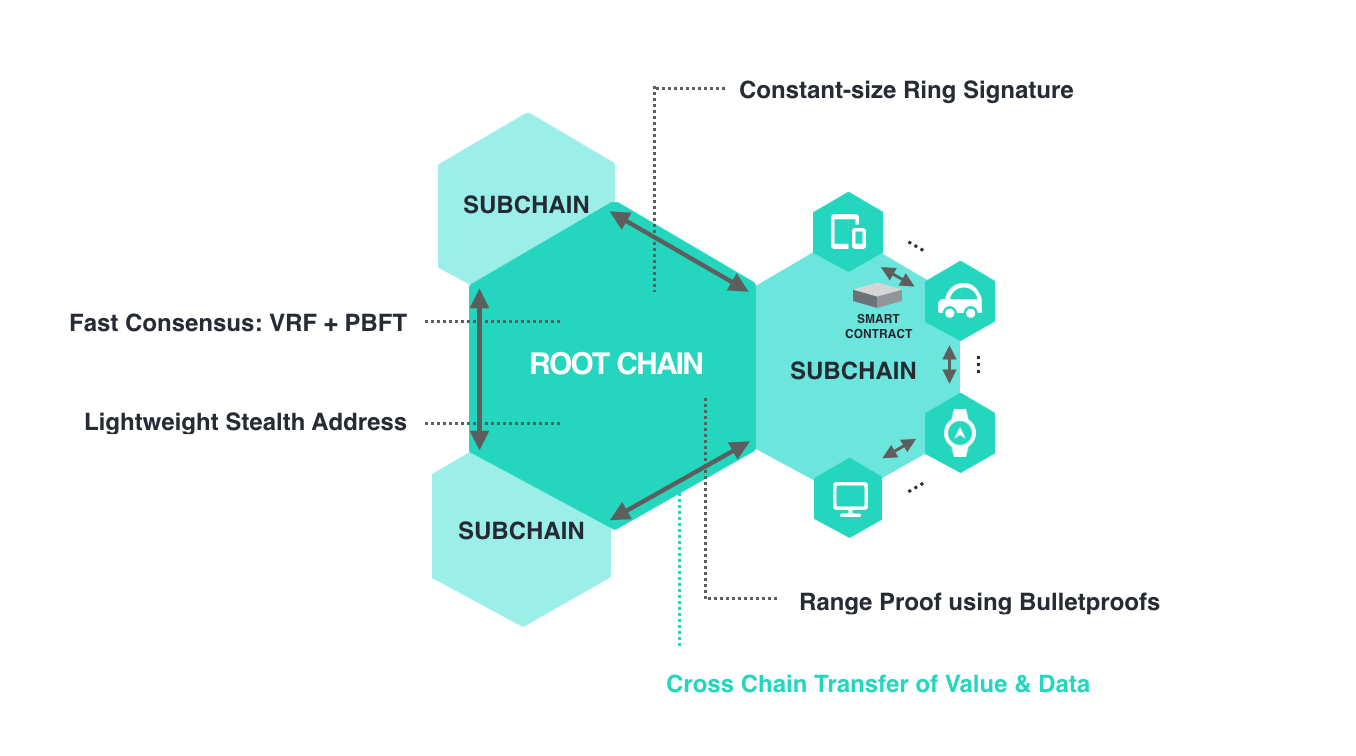
\includegraphics[width=\textwidth]{Figura1.png}
	\label{fig:fig1}
	\caption{IoTeX: Blockchain in blockchain, una architettura di rootchain con subchain}
\end{figure}

La blockchain radice è una blockchain pubblica accessibile da chiunque, che ha tre obiettivi principali:

\begin{enumerate}
	\item
	      \textbf{Inoltro} di valore e dati tra le subchain in modo da preservare la privacy per abilitare l'interoperabilità tra le subchain;
	\item
	      \textbf{Supervisione} delle subchain, ad esempio penalizzare gli operatori di subchain confiscando il deposito;
	\item
	      \textbf{Regolamento e ancoraggio} dei pagamenti e della fiducia per le subchain.
\end{enumerate}
Con questi obiettivi definiti, la rootchain si concentra in particolare su scalabilità, robustezza,
funzioni per preservare la privacy e capacità di controllare le subchain.
Una subchain, d'altra parte, potrebbe potenzialmente essere una blockchain privata e dipendere dalla rootchain per l'interazione con altre sottocatene. Una subchain richiede flessibilità
ed estendibilità per adattarsi ai diversi requisiti delle diverse applicazioni IoT. Una subchain sarà molto probabilmente gestita da operatori il cui ruolo è subordinato a un deposito di garanzia sufficiente, depositato sulla rootchain. Opzionalmente, il sistema consente agli operatori di nominare uno o più operatori che agiscono per suo conto, con o senza vincoli extra. L'operatore agisce come un client leggero nella rootchain, e come un nodo completo nella subchain per
confermare nuovi blocchi.
Nel complesso, le proprietà di rootchain e subchain sono riassunte in Tabella \ref{table:rootchainandsubchains}

\begin{table}[tp]%
	\caption{Confronto tra Rootchain e Subchain}
	\label{table:rootchainandsubchains}\centering %
	\begin{tabular}{l|l|l}
		\hline
		\textbf{Proprietà}          & \textbf{Rootchain}   & \textbf{Subchain}  \\
		\hline
		Pubblica vs Privata         & Pubblica             & Pubblica o Privata \\
		Scalabile                   & Necessario           & Varia              \\
		Robusta                     & Fortemente Richiesto & Richiesto          \\
		Incentrata sulla Privacy    & Richiesto            & Varia              \\
		Estendibilità               & Non-Turing completa  & Turing completa    \\
		Finalità Istantanea Blocchi & Richiesta            & Richiesta          \\
		\hline
	\end{tabular}
\end{table}

\subsection{Blockchain Root}
La blockchain root utilizza il modello basato su UXTO come Bitcoin \cite{c21} e Monero \cite{c20} per i seguenti motivi:

\begin{itemize}
	\item
	      L'ordinamento delle transazioni diventa banale, senza richiedere \emph{nonce} o
	      numeri di sequenza, il che pone richieste minime sugli schemi di consenso e permette di elaborare le transazioni in parallelo;
	\item
	      Applicando tecniche esistenti di conservazione della privacy come \emph{ring signature} e ZKSNARKs, diventa possibile nascondere il mittente, il destinatario e l'importo della transazione;
\end{itemize}

La blockchain radice è composta da blocchi collegati da hash, ed un blocco è costituito da  un'intestazione lo collega mediante un hash al blocco precedente, e da un elenco di transazioni.
La rootchain consente principalmente due tipi di transazione: (1) transazioni di base incluse
\texttt{P2PKH, P2SH, Multisig} e così via, e transazioni avanzate che consentono
operazioni tra blockchain come \texttt{BondedRegistration, Lock, ReLock, Reorg} ecc.. Le
transazioni validate vengono aggiunte ad un blocco che ha dimensione dinamica, con limite superiore di 8MB. Il nostro sistema di consenso produce un blocco ogni tre secondi come dettagliato
nella prossima sezione. La rootchain è progettata per essere non-Turning-Completa con il
supporto di uno script basato su stack e un ricco set di operazioni.

\subsection{Subchain}
IoTeX dispone di un framework per lo sviluppo e la fornitura di una subchain su misura
per applicazioni IoT decentralizzate incapsulando primitive a basso livello come il protocollo gossip
ed il meccanismo di consenso. Il modello di autorizzazione, le specifiche, i parametri,
e i tipi di transazione della subchain possono essere personalizzati per adattarsi alla sua applicazione.
Le subchain IoTeX utilizzano il modello basato sull'account, che è migliore per il tracciamento delle transizioni di stato.
Esistono due tipi di account, similmente a Ethereum, account regolari e
contratti. Le transazioni valide vengono aggiunte al blocco, che viene generato dallo stesso
schema di consenso della catena principale per raggiungere lo stesso livello di finality per rendere la comunicazione cross-chain più efficiente. Le subchain possono sia utilizzare il token della rootchain, IoTeX, oppure definire il proprio token. Il token definito dagli sviluppatori per le subchain possono essere distribuiti mediante vendita pubblica di token oppure scambiati sugli exchange pubblici.
Le subchain supportano smart contract, che vengono eseguiti su una macchina virtuale leggera ed efficiente. Attualmente stiamo valutando Web Assembly (WASM) \cite{c36}, uno standard Web emergente per la creazione di applicazioni Web ad alte prestazioni. WASM è veloce ed efficiente, può essere reso deterministico e dotato di sandbox a seguito di piccole modifiche così come tentato dal progetto EOS \cite{c9}. Anche altre opzioni vengono esplorate. Grazie agli smart contract, i dispositivi IoT collegati alla stessa subchain usano lo stato condiviso in due modi,

\begin{itemize}
	\item Innanzitutto, i dispositivi possono interagire con l'ambiente fisico in base agli stati delle loro subchain, ad es. le lampadine si accendono o spengono autonomamente in base allo stato di un orologio sulla stessa subchain;

	\item D'altra parte, i dispositivi possono cambiare il proprio stato sulla subchain quando
	      quando l'ambiente fisico cambia, ad esempio, il termostato aggiorna la temperatura tramite uno smart contract in base ai dati provenienti dal suo sensore;
\end{itemize}

\subsection{Comunicazione cross-blockchain}
Ci si aspetta che la comunicazione tra blockchain diverse sarà utilizzata di frequente nelle applicazioni in IoT. C'è sempre la necessità per un dispositivo IoT in una subchain di coordinarsi con un altro dispositivo in una diversa subchain. Ancora una volta, limitati dalla bassa potenza di calcolo e dal poco spazio di archiviazione dei dispositivi IoT, siamo motivati a progettare un tipo di comunicazione cross-blockchain che sia rapida ed economica in termini di risorse.

\subsubsection{Pegging e Finalità dei blocchi}
Il Pegging è un meccanismo per scalare la rete Bitcoin tramite \emph{"sidechain"}, originariamente
proposto in \cite{c1}. Esso si affida fortemente al \emph{Simplified Payment Verifcation} (SPV) \cite{c21}, e consente ai Bitcoin di \"spostarsi\" in modo efficiente dalla blockchain Bitcoin a una sidechain
e viceversa. L'idea alla base è semplice: i token vengono inviati ad un indirizzo speciale al fine di essere bloccati sulla blockchain Bitcoin; una volta confermata questa transazione di \texttt{Lock}, si invia la transazione \texttt{Reorg} alla sidechain, includendo la transazione \texttt{Lock} ed una
prova di inclusione (\emph{"Proof of inclusion"}), sotto forma di ramo Merkle. La sidechain usa SPV per verificare la transazione di \texttt{Reorg} e, se convalidata, crea una quantità di token equivalente e li invia all'indirizzo desiderato sulla sidechain. Ad oggi, il pegging funge da
primitiva per quasi tutti i protocolli di comunicazione cross-blockchain, ad es. Cosmos, Lisk,
Rootstock. Due flussi separati di pegging possono essere facilmente accoppiati insieme per creare il
cosiddetto Pegging a due vie (2WP) per renalizzare il trasferimento di token in entrambi i versi.

La finalità dei blocchi è la garanzia che ogni nuovo blocco generato sia "finale", e non può più essere
cambiato. La finalità dei blocchi ha un impatto sostanziale sull'attuazione concreta del pegging,
poiché è necessario aspettare fino a che la finalità di un blocco venga raggiunta (almeno con alta flessibilità) sulla blockchain da cui si invia prima di richiedere la \texttt{Reorg}. La maggior parte delle blockchain pubbliche come Bitcoin non hanno finalità istantanea. La blockchain ricevente può ottenere solo una assicurazione statistica, poiché man mano che più miners PoW confermano una transazione, aumenta la probabilità che essa sia stata accettata. Utilizzare un consenso con finalità risolve questo problema perché la blockchain ricevente ha la garanzia già con la conferma di un solo blocco sulla blockchain da cui si invia. Per le applicazioni IoT, il trasferimento tra le blockchain di valore e dati dovrebbe essere veloce e richiedere poche risorse, il che richiede un meccanismo di consenso con finalità sia sulla rootchain che sulle subchain. Il consenso IoTeX raggiunge la finalità istantanea dei blocchi, come dettagliato nella prossima sezione.

\subsubsection{Protocollo di comunicazione cross-blockchain}
Esaminiamo il protocollo ad un alto livello immaginando che un indirizzo di nome Charlie sulla
subchain 1 desideri inviare una transazione a un indirizzo chiamato David sulla subchain 2, e tutte e tre le blockchain usino lo stesso tipo di token, per semplicità senza costi di transazione. Si noti che applicando semplicemente il pegging, saranno necessarie quattro transazioni per effettuare una "remote call" dalla subchain 1 alla subchain 2 attraverso la rootchain, cioè, (1) una transazione di \texttt{Lock} sulla subchain 1; (2) una transazione di \texttt{Reorg} verso la rootchain; (3) un'altra transazione di \texttt{Lock} sulla rootchain; e (4) un'altra transazione di \texttt{Reorg} verso la subchain 2.
Questo processo indica che David deve attendere almeno 4 blocchi prima di accettare questa "remote call", e i dati che questa "remote call" trasporta devono essere archiviati su tutte e tre le blockchain, e ciò la rende lenta e costosa. Miriamo a ottimizzare questo processo combinando (2)
e (3) in un'unica transazione di \texttt{ReLock}, che non solo accelera l'intero processo ma
evita anche di archiviare i dati nella subchain 1 e nella rootchain. Il nostro protocollo è raffigurato
nella Figura \ref{fig:fig2}

\begin{figure}[ht]
	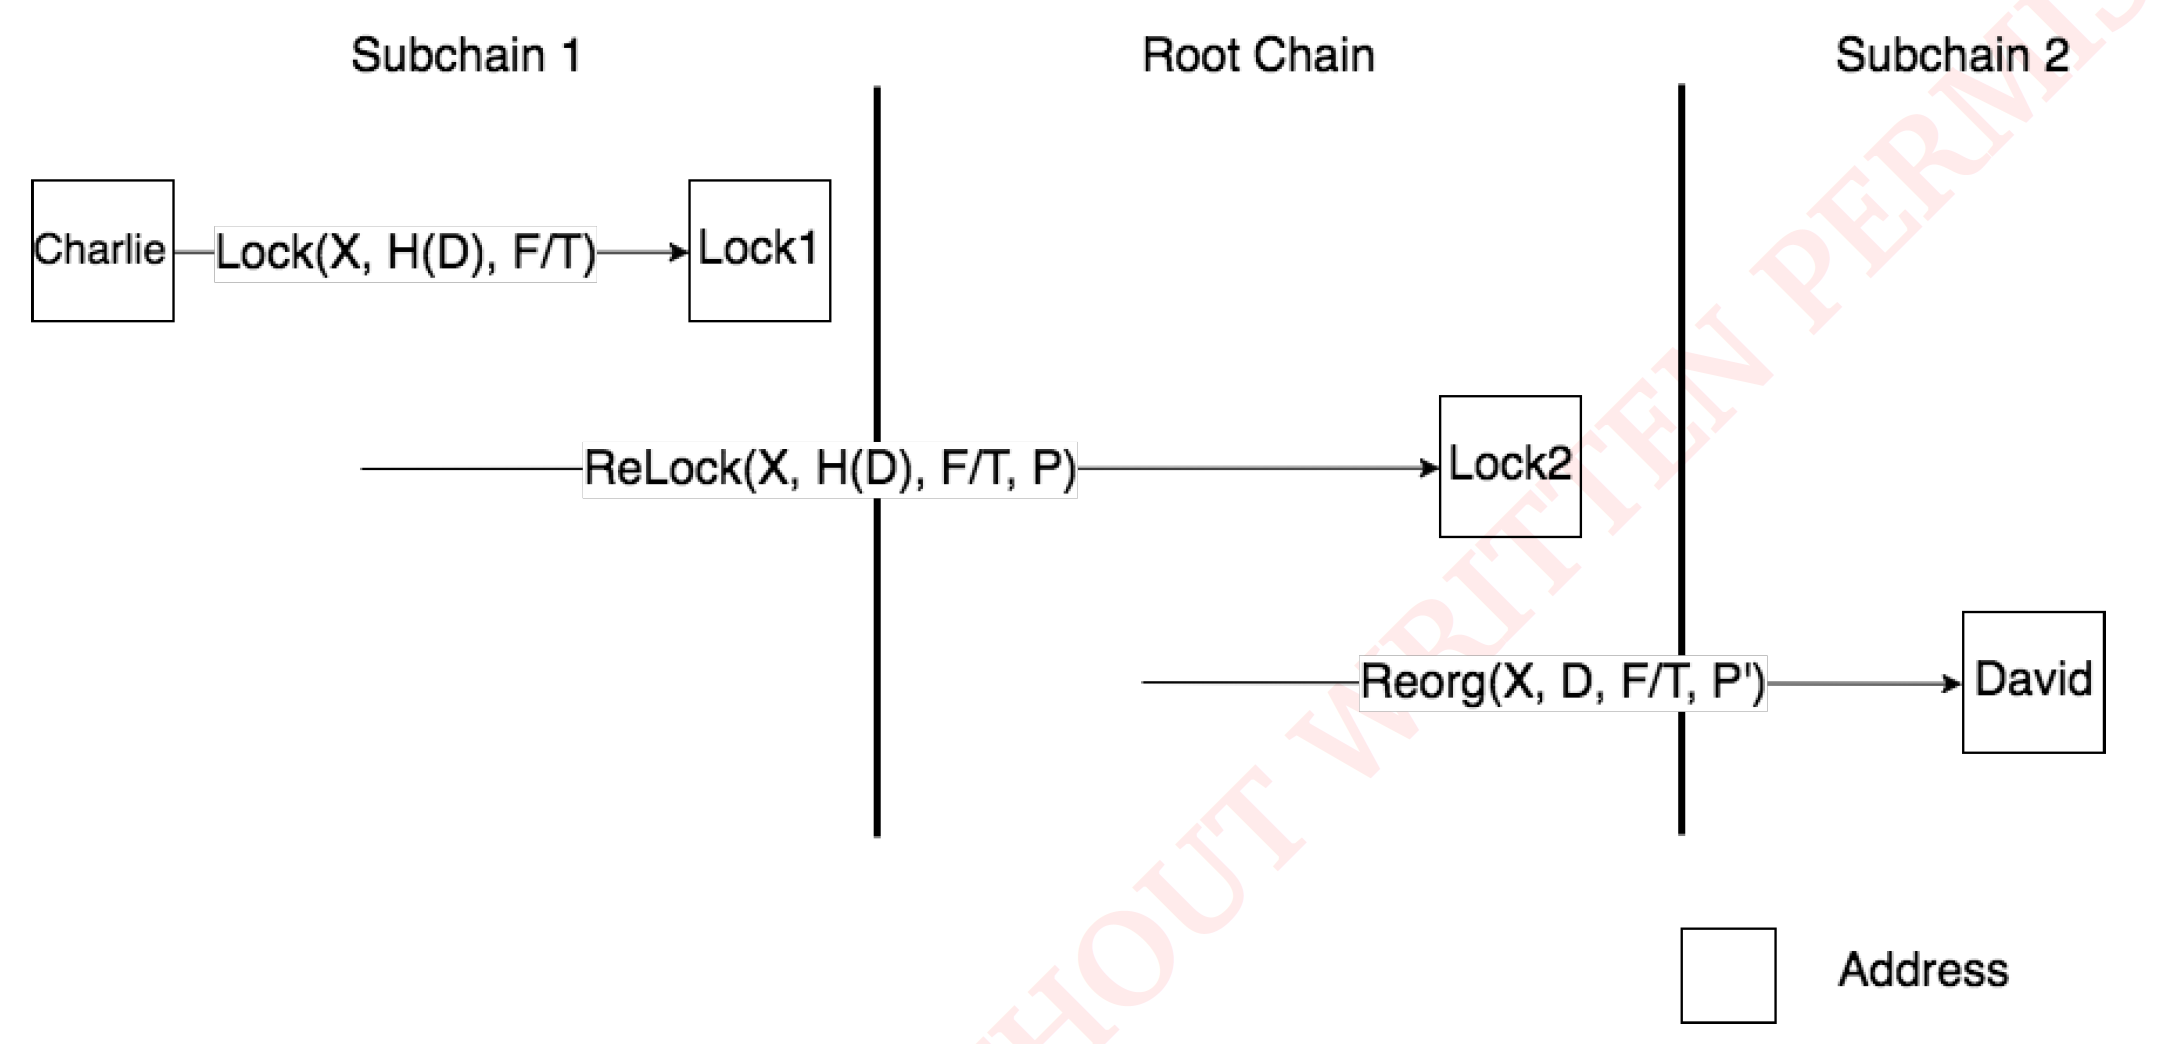
\includegraphics[width=\textwidth]{Figura2.png}
	\label{fig:fig2}
	\caption{Transazioni Cross-Bockchain}
\end{figure}

Il protocollo Cross-Blockchain di IoTeX è composto dai seguenti passi:

\begin{itemize}
	\item Ogni subchain viene registrate sulla rootchain inviando una transazione chiamata \texttt{BondedRegistration} alla rootchain, che include il nome della subchain, l'ID, la configurazione, il blocco "genesis", e la nomenclatura degli operatori; questo processo avviene una sola volta;

	\item Quando Charlie vuole inviare una transazione a David, inizia una transazione $\texttt{Lock}(X, H(D), F/T)$ dove $X$ è la quantità di token, $H(D)$ è l'hash dei dati $D$ da allegare, $F/T$ indica gli indirizzi sorgente e destinazione inclusi gli ID per entrambe le subchain;

	\item Una volta che la transazione di \texttt{Lock} è stata inclusa nella blockchain 1, Charlie inizia una transazione $\texttt{ReLock(X, H(D), F/T, S, P)}$ con la rootchain includendo $X, H(D), F/T$, alcune statistiche correnti della subchain 1 indicati con $S$ e una "\emph{proof-of-inclusion}" $P$ che comprende i rami Merkle delle intestazioni di blocchi recenti e rami Merkle che provano che la transazione \texttt{Lock} è stata inclusa;

	\item La rootchain valida la transazione \texttt{ReLock} e la accetta includendola nell'ultimo blocco, e crea $X$ token bloccandoli in un indirizzo speciale;

	\item Una volta che la transazione \texttt{ReLock} è stata inclusa nella rootchain, Charlie invia una transazione $\texttt{Reorg}(X, D, F/T, P')$ sulla rete della rootchain con $X, D, F/T$ ed un'altra \emph{proof-of-inclusion} $P'$ che prova l'inclusione della transazione \texttt{ReLock};

	\item Gli operatori della subchain 2 si accorgono della transazione \texttt{Reorg}, dunque validano e creano la stessa quantità di token sulla subchain 2 inviandoli all'indirizzo di David con associati i dati $D$.

\end{itemize}

\subsubsection{Condivisione della larghezza di banda della Blockchain Root}
Una possibile proeccupazione che riguarda la comunicazione cross-blockchain, è che subchain malevoli possano fare \emph{spam} sulla rootchain o un'altra subchain trasmettendo un'enorme quantità di transazioni cross-blockchain esaurendo la capacità dell'altra blockchain. Un modo di attenuare il problema è di lasciare che ogni subchain appalti la propria quota e limiti la frequenza delle transazioni da provenienti una subchain se la propria quota si esaurisce.

\begin{figure}[ht]
	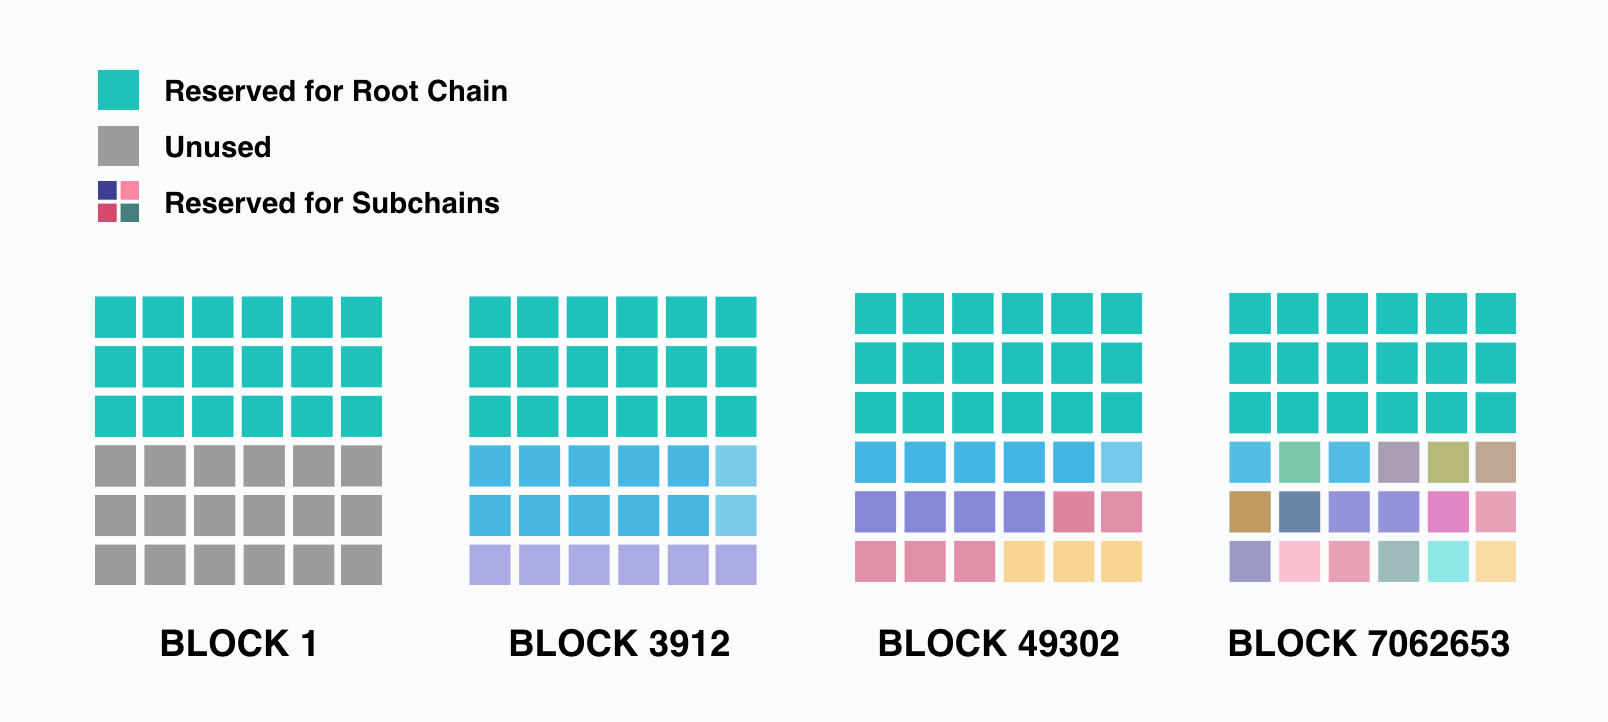
\includegraphics[width=\textwidth]{Figura3.png}
	\label{fig:fig3}
	\caption{Modello della Largezza di Banda per Sondividere la Capacità della Rootchain}
\end{figure}

Si potrebbe definire una quota basandosi sullo spazio all'interno di un blocco. Supponiamo che la dimensione massima di un blocco sia di 8MB, e che 4MB siano riservati per le normali transazioni all'interno della rootchain, e 4MB siano riservati per tutte le transazioni cross-blockchain, ulteriormente suddivisi in, diciamo 4096 parti di quota, con ogni parte di 1KB. Una subchain richiede l'allocazione $n$ parti di quota (con un limite massimo fissato) per gli usi desiderati, versando una cauzione proporzionale ad $n$. Ad ogni round, solo $n$KB possono essere occupati all'interno di ciascun blocco per le transazioni provenienti da quella subchain e per ognuna di esse viene scalata una "commissione di banda" dal deposito (per premiare i miner che aiutano ad applicare questa regola); le transazioni rimanenti vengono accodate e, alla fine, scartate quando scadono. L'allocazione delle quote può essere dinamica nel senso che subisce cambiamenti quando la rootchain cresce, come mostrato in Figura \ref{fig:fig3}. Se una subchain inviasse spam alle altre, consumerebbe il proprio deposito molto velocemente ed alla fine perderebbe la propria quata di banda. D'altra parte, se una subchain versasse un grosso deposito esclusivamente al fine di riservare una gran parte di larghezza di banda senza in realtà utilizzarla, la rootchain avrebbe un meccanismo per risarcire perte del deposito secondo il rapporto tra il numero medio di transazioni per blocco e la porzione di banda riservata, il che aiuta a stabilizzare la larghezza di banda riservata ad un valore vicino a quella attualmente utilizzata.

\section{Transazioni con Protezione della Privacy Integrata}
La privacy fornita in modo nativo da Bitcoin ed Ethereum è limitata alla pseudonimia, mentre i dettagli della transazione non sono riservati. L'importo della transazione ed i beni trasferiti, i loro metadati e le relazioni con altre transazioni possono essere  banalmente verificate da chiunque. In effetti, in questo contesto, esistono tre aspetti della privacy: la privacy del mittente, la privacy del destinatario e la privacy dei dettagli della transazione. Vari metodi crittografici possono essere applicati per affrontarli, come mostrato nella Tabella \ref{table:PrivacyPreservingTechniques}.

\begin{table}[tp]%
	\caption{Tecniche di Conservazione della Privacy per le Blockchain}
	\label{table:PrivacyPreservingTechniques}\centering %
	\begin{tabular}{l|p{2cm}c|p{2.5cm}|p{2cm}}
		\hline
		Tecnica              & Nasconde il Mittente & Nasconde il destinatario & Nasconde l'Importo \\
		\hline
		Stealth Address      & N                    & Y                        & N                  \\
		Pedersen Commitments & N                    & N                        & Y                  \\
		Ring Signatures      & Y                    & N                        & N                  \\
		zk-SNARKs            & Y                    & N                        & Y                  \\
		\hline
	\end{tabular}
\end{table}

IoTeX integra lo stealth address per la privacy del destinatario, la ring signature per la privacy del mittente, ed il Pedersen Commitments per nascondere l'importo della transazione, con le seguenti innovazioni e miglioramenti:

\begin{itemize}
	\item Un algoritmo di stealth address leggero, progettato per sollevare i destinatari dall'onere di scandire l'intera blockchain per venire a conoscenza delle transazioni in arrivo;

	\item Una ring signature ottimizzata per ridurne le dimensioni, senza utilizzare una configurazione distribuita di tipo trusted.
\end{itemize}


\subsection{Nascondere il destinatario della transazione mediante Codice di Pagamento Inoltrabile}

\subsubsection{Stealth Address}
La tecnica dello stealth address nasce dal protocollo Cryptonote \cite{c28}, che risolve il problema del destinatario utilizzando un protocollo di scambio di chiavi Diffie-Hellman a "mezzo giro". Supponendo che \emph{Bob} voglia nascondere il fatto che riceverà dei token da \emph{Alice}, ecco come funzionerebbe:

\begin{enumerate}
	\item \emph{Bob} crea due coppie di chiavi private e pubbliche, indicate come $(a, A)$ e $(b, B)$, dove $A = a\cdot G$, $B = b\cdot G$, e $G$ è il punto base su una curva ellittica.

	\item \emph{Bob} divulga le chiavi pubbliche $(A, B)$, note come il suo "stealth address";

	\item \emph{Alice} calcola e invia i token a $P = H (rA)\cdot G + B$ usando una funzione hash $H$, un numero casuale e grande $r$  e lo stealth address di \emph{Bob} $B$. Questa transazione viene trasmessa insieme a $R = r\cdot G$;
	\item  \emph{Bob} monitora tutte le transazioni, calcola $P' = (H(aR) + b)\cdot G$ (poiché egli conosce $a$, $b$, $R$ e $G$) con la speranza che $P'$ sia uguale a $P$. Se $P' = P$, Bob potrà spendere i token inviati a $P'$ con la chiave privata $H(aR) + b$.
\end{enumerate}

Un inconveniente evidente dello stealth address è che il destinatario deve monitorare tutte le transazioni della rete (il che non è l'ideale nel mondo IoT), oppure in alternativa deve basarsi sull'assistenza di un full-node di fiducia che lo faccia per lui (il che a un certo livello compromette la privacy).

\subsubsection{Codice di pagamento}
Il codice di pagamento è stato ideato per risolvere l'inconveniente di cui sopra relativo allo stealth address, sacrificando in parte la privacy. L'idea è che \emph{Alice} notifichi a \emph{Bob} un codice di pagamento tramite un metodo riservato, e Bob monitori solo le transazioni verso gli indirizzi derivanti da quel codice. Pertanto, questa proposta presenta due flussi: quello della notifica, che rappresenta una configurazione una-tantum tra certe due parti, e quello di invio, che può accadere più volte tra queste due parti.

Supponendo che \emph{Alice} abbia una coppia di chiavi pubblica-privata principali ($mpub_{Alice}, mpri_{Alice}$) dove $mpub_{Alice} = mpri_{Alice}\cdot G$, ed una coppia di chiavi pubblica-privata di portafoglio ($wpub_{Alice}, wpri_{Alice}$) dove $wpub_{Alice} = wpri_{Alice}\cdot G$; che \emph{Bob} abbia una coppia di chiavi pubblica-privata principali $(mpub_{Bob}; mpri_{Bob})$ dove $mpub_{Bob} = mpri_{Bob}\cdot G$, la notifica una tantum funziona come descritto di seguito:

\begin{enumerate}
	\item \emph{Bob} deriva $B_0 = b_0\cdot G = (mpri_{Bob} + Hash(0, seed, metadata))\cdot G$, lo converte in un indirizzo di notifica $\texttt{addr}(B_0)$, lo pubblica e si mette in ascolto su di esso

	\item  \emph{Alice} sceglie un codice $cc$ a caso; $(mpub_{Alice}||cc)$ è il codice di pagamento per \emph{Alice};

	\item  \emph{Alice} calcola un codice segreto condiviso $S = wpri_{Alice}\cdot B_0$ ed invia il codice di  pagamento mascherato $P' = (mpub_{Alice}||cc)\oplus HMAC512(xofS)$ ad $\texttt{addr}(B_0)$;

	\item Alla ricezione, \emph{Bob} ottiene $wpub_{Alice}$ e recupera $S = wpub_{Alice}\cdot b_0$, scopre $P'$ per ottenere $(mpub_{Alice}||cc)$.
\end{enumerate}

Una volta che il flusso di notifica è completo, \emph{Alice} e \emph{Bob} stabiliscono un canale privato unidirezionale per l'invio di token. Il primo invio funziona come descritto di seguito:

\begin{enumerate}
	\item \emph{Alice} deriva un nuovo indirizzo dal suo codice di pagamento (che è già condiviso con \emph{Bob}) da $A_0 = a_0\cdot G = mpub_{Alice} + Hash(0, seed, metadata)\cdot G$;

	\item \emph{Alice} seleziona la successiva chiave pubblica non ancora utilizzata, derivata da $B_0$. Si noti che $B_0$ è la chiave pubblica inutilizzata per il primo round.

	\item \emph{Alice} calcola il nuovo codice segreto condiviso $S_0 = a_0\cdot B_0$ e calcola la chiave pubblica temporanea utilizzata per inviare la transazione per cui si verifica $B'_0 = B_0 + SHA256(S_0)\cdot G$

	\item \emph{Bob} potrebbe derivare $A_0$ in modo non interattivo poiché conosce il codice di pagamento di Alice, e ascolta solo l'indirizzo derivato da $B'_0 = B_0 + SHA256(S_0)\cdot G$ ed $S_0 = A_0\cdot b_0$.

	\item Alla ricezione, \emph{Bob} può spendere i token con la chiave privata $b_0 + SHA256(S_0)$.

\end{enumerate}

I flussi successivi funzionano in maniera analoga.
\emph{Bob} non ha bisogno di monitorare la rete o affidarsi a un full-node per eseguire la scansione di tutte le transazioni. La transazione di notifica fa trapelare l'intenzione di \emph{Alice} di inviare qualcosa a \emph{Bob}, ma l'effettivo "invio di qualcosa" è nascosto a tutti gli altri.

\subsubsection{Codice di Pagamento Inoltrabile}
Per ridurre ulteriormente la perdita di privacy, abbiamo progettato il \emph{codice di pagamento inoltrabile} basandoci sulla proposta originaria del \emph{codice di pagamento} appena descritta. Mentre il flusso di invio rimane lo stesso, abbiamo migliorato il flusso di notifica per consentire ad \emph{Alice} di condividere segretamente il suo codice di pagamento con \emph{Charlie} senza utilizzare la transazione di notifica, assumendo che \emph{Alice} e \emph{Bob} abbiano un canale privato unidirezionale, e \emph{Bob} e \emph{Charlie} abbiano un altro canale privato unidirezionale. Per ottenere ciò, sfruttiamo i contratti Hashed Timelock (HTLC - \emph{Hashed TimeLock Contracts}), i quali richiedono che il destinatario di un pagamento confermi la ricezione di un pagamento prima di una deadline, generando una dimostrazione di pagamento (\emph{proof of payment}) crittografata, oppure rinunci alla possibilità di reclamare il pagamento, restituendolo al mittente.


Supponendo che \emph{Charlie} abbia una coppia di chiavi pubblica-privata $(mpub_{Charlie}, mpri_{Charlie})$ dove $mpub_{Charlie} = mpri_{Charlie}\cdot G$. Il flusso di notifica migliorato funziona come illustrato di seguito:

\begin{enumerate}
	\item \emph{Charlie} deriva $C_0 = c_0\cdot G = (mpri_{Charlie} + Hash(0, seed, metadata))\cdot G$, lo converte in un indirizzo di notifica $\texttt{addr}(C_0)$, lo pubblica. Si noti che $C_0$ è pubblicato per \emph{Alice} al fine calcolare il codice segreto condiviso, ma non per ricevere transazioni;

	\item \emph{Alice} genera il suo codice di pagamento $(mpub_{Alice}||cc)$ nello stesso modo;

	\item \emph{Alice} calcola un codice segreto condiviso $S = wpri_{Alice}\cdot C_0$ e invia il codice di pagamento mascherato $P' = (mpub_{Alice}||cc) \oplus HMAC512(xofS)$ con $X$ token come incentivo e $HTLC(Hash^2(cc))$ a \emph{Bob} usando il loro canale privato unidirezionale, dove $HTLC$, come parte dello script di blocco o riscatto, afferma che i token diventano
	      spendibili se viene fornita la pre-immagine di $Hash^2(v)$, ovvero $Hash (cc)$;

	\item \emph{Bob}, incentivato dai token inviati da Alice, invia $P'$, $Y$, $Y < X$ token ed $HTLC(Hash^2(v))$ a \emph{Charlie} usando il loro canale privato unidirezionale;

	\item \emph{Charlie}, dopo aver ricevuto la transazione di \emph{Bob}, calcola $S = wpub_{Alice}\cdot c_0$ per scoprire il codice di pagamento di \emph{Alice}, e spendere la transazione rivelando $Hash(cc)$, che rende spendibile la transazione da \emph{Alice} a \emph{Bob}, e che premia \emph{Bob}.
\end{enumerate}

Una volta che questo flusso viene completato, \emph{Alice} e \emph{Charlie} stabiliscono un canale privato unidirezionale per l'invio di token. È interessante notare che il tragitto della transazione di \emph{Alice} potrebbe consistere di più salti.

I nostri codici di pagamento inoltrabili offrono una privacy maggiore in termini di occultamento dell'intenzione di "inviare qualcosa" sulla blockchain, sfruttando i canali privati esistenti, e senza aggiungere alcun overhead di elaborazione o di archiviazione per i nodi. Inoltre, sebbene progettati per scenari IoT, i codici di pagamento inoltrabili risultano utilizzabili per la maggior parte delle blockchain come Bitcoin.

\subsection{Abilitare Transazioni Riservate}

\subsubsection{Definizione del Problema}
In Figura \ref{fig:fig4} viene mostrata una tipica transazione sulla blockchain Bitcoin. In sostanza, una transazione blockchain è semplicemente una tupla $({pk_{in,i}, {pk_{out,j},{v_{i,j}}}})$, dove $({pk_{in,i}})$ rappresentano indirizzi di input, ${pk_{out,j}}$ indirizzi di output, e ${v_{i,j}}$ sono gli importi delle transazioni tra gli indirizzi di input e output. Poiché le transazioni Bitcoin sono memorizzate in chiaro in un registro pubblico, ciò ha sollevato molti problemi in termini di sicurezza e privacy.

\begin{figure}[ht]
	\centering
	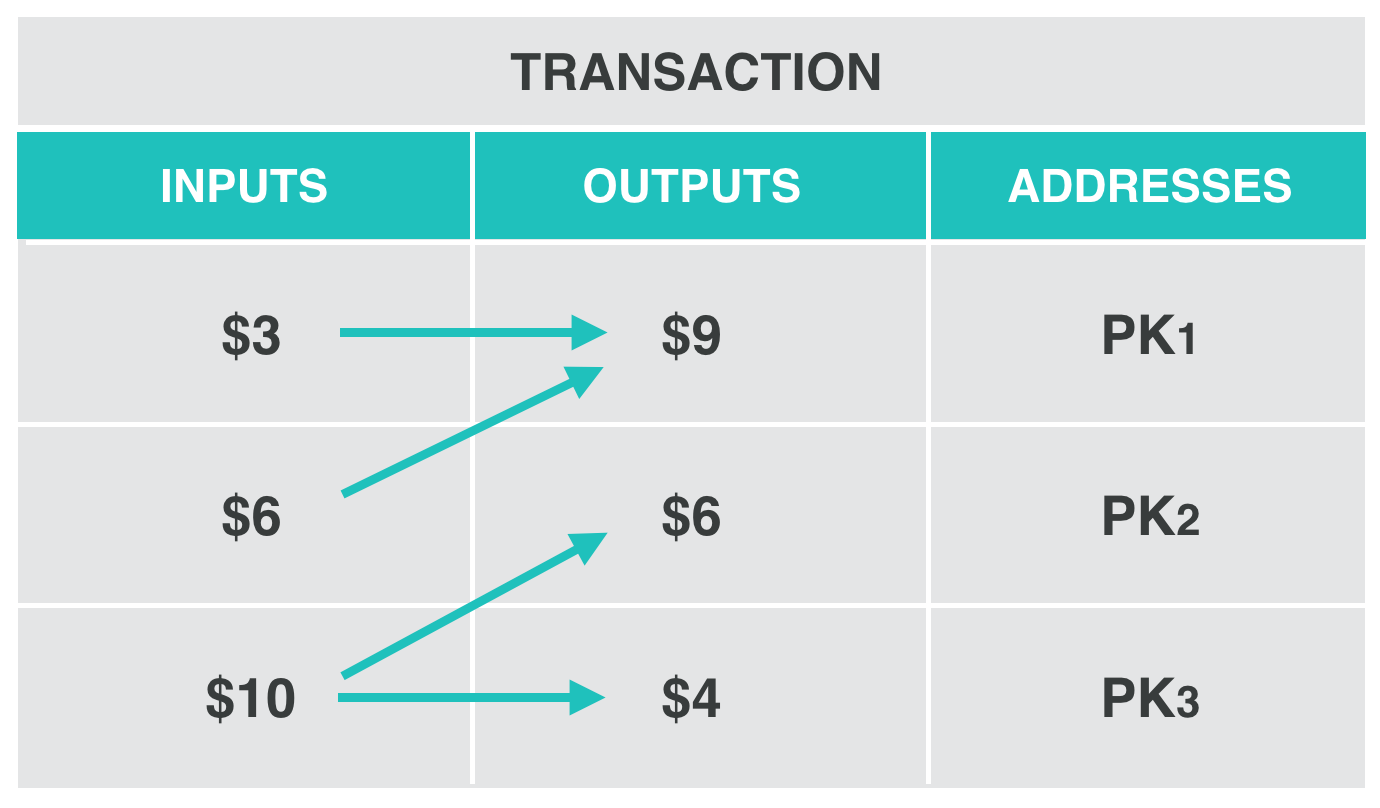
\includegraphics[width=0.5\textwidth]{Figura4.png}
	\caption{Una transazione sulla Blockchain Bitcoin}
	\label{fig:fig4}
\end{figure}

L'obiettivo delle transazioni riservate (vedere la Figura \ref{fig:fig5}) è quello di consentire solo ai mittenti e ai destinatari delle transazioni di rivelarne il valore ${v_{i,j}}$ e di nasconderlo al resto del mondo. Inoltre, le transazioni riservate consentono comunque alle altre entità della rete di verificare la validità di tali transazioni, pur senza poter vedere gli importi effettivi. La realizzazione di transazioni riservate su blockchain richiede un certo numero di tecniche crittografiche avanzate.

\begin{figure}[ht]
	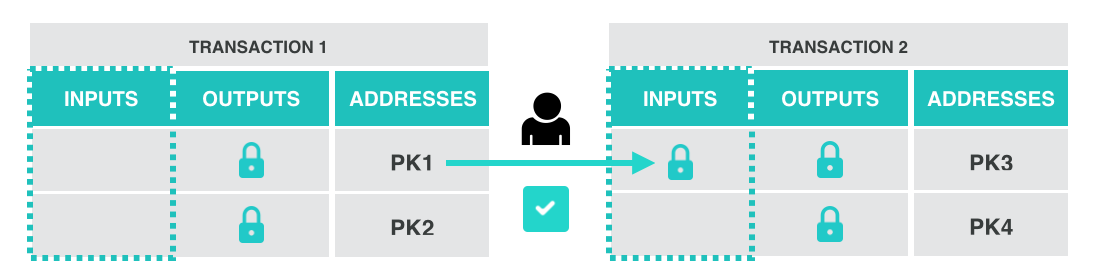
\includegraphics[width=\textwidth]{Figura5.png}
	\label{fig:fig5}
	\caption{Una transazione Riservata Con Verificabilità Pubblica}
\end{figure}

\subsubsection{Prova di Conoscenza}
Una prova di conoscenza (\emph{proof of knowledge}), indicata con $(P, V)$, è una dimostrazione interattiva tra un dimostratore $P$ ed un verificatore $V$, in cui il dimostratore vuole dimostrare di conoscere alcune informazioni. In particolare, $P$ possiede $(x, w)$ legati da una relazione $R$, dove $x$ è il problema e $w$ è la soluzione (anche detta \emph{testimone}). $V$ conosce $x$, e confermerà solo se $P$ riesce a convincere $V$ che egli conosce $w$.

\subsubsection{Dimostrazione a conoscenza zero}
In un protocollo a conoscenza zero (\emph{zero-knowledge}), il dimostratore dimostra un'affermazione al verificatore, senza rivelare nient'altro sull'affermazione oltre alla veridicità della stessa, cosa che protegge il dimostratore da verificatori malevoli che cerchino di acquisire più informazioni del necessario. Il protocollo può essere \emph{interattivo} o \emph{non interattivo}. La differenza chiave delle dimostrazioni non interattive è che tutte le interazioni consistono in un singolo messaggio inviato dal dimostratore al verificatore. Usiamo la notazione $\texttt{NIZKPoK}(\alpha, \beta): a = g^{\alpha} \wedge b = g^{\beta}$ per denotare una prova a conoscenza zero dei valori $\alpha$ e $\beta$ non interattiva, tale che $a = g^{\alpha} e b = g^{\beta}$. Si presume che tutti i valori non racchiusi tra parentesi siano noti al verificatore. Quando usiamo una dimostrazione a conoscenza zero non interattiva per autenticare dati ausiliari, lo schema risultante è indicato come \emph{firma di conoscenza} ("\emph{Signature of Knowledge}")\cite{c8}. Fondamentalmente, uno schema a firma di conoscenza significa che un soggetto in possesso di una soluzione $w$ al problema $x$ ha firmato il messaggio $m$. Per il \texttt{NIZKPoK} di cui sopra, usiamo la notazione $\texttt{SoK}[m](\alpha, \beta): a = g^{\alpha} \wedge b = g^{\beta}$ per indicare una firma di conoscenza sul messaggio $m$.

\subsubsection{Ring Signature}
Il concetto di firma ad anello (\emph{"Ring Signature"}) è stato introdotto per la prima volta da Rivest et al. \cite{c27} nel 2001 come un tipo particolare di firma di gruppo. In una firma ad anello, il firmatario del messaggio seleziona un insieme di membri dell'anello, compreso se stesso, come possibili firmatari di messaggi. Il verificatore può essere convinto che la firma sia stata effettivamente generata da uno dei membri dell'anello.
Tuttavia, il verificatore non è in grado di stabilire quale membro abbia effettivamente generato la firma. A differenza di una firma di gruppo generica, uno schema di firma ad anello non comporta la scelta di un manager del gruppo per la gestione dell'insieme dei membri dell'anello, eliminando in tal modo la possibilità che l'identità del vero firmatario del messaggio possa essere rivelata dal manager del gruppo. Al fine di garantire l'anonimato nelle transazioni di token mediante smart contract, nella criptovaluta Monero è stato utilizzato un tipo speciale di firma ad anello, la cosiddetta firma ad anello collegabile \cite{c20}. La firma ad anello collegabile ha la proprietà aggiuntiva per cui qualunque firma generata dallo stesso firmatario, sia che firmi lo stesso messaggio o messaggi diversi, ha un identificatore (chiamato tag) che collega le firme. Questa proprietà consente a terzi di verificare in modo efficiente che le firme sono state generate dallo stesso soggetto, senza divulgarne l'identità. La firma ad anello collegabile utilizzata in Monero viene chiamata  Multi-Layered Linkable Spontaneous Anonymous Group Signature (MLSAG)\cite{c22}, che è una firma ad anello su un insieme di vettori di chiavi ed ha una complessità di comunicazione di $O(m(n + 1))$, dove $m$ è il numero di coppie di chiavi pubbliche/private di proprietà del firmatario ed $n$ è la dimensione dell'anello.

\subsubsection{Accumulatore}
Gli accumulatori unidirezionali, che furono proposti per la prima volta da Benaloh e de Mare in \cite{c2}, sono definiti come funzioni hash unidirezionali con la proprietà di essere \emph{quasi-commutative}. Una funzione quasi-commutativa $f: X \times Y \Rightarrow X$ è tale che, per ogni $x \in X$ e per ogni $y_1, y_2 \in Y$, abbiamo che $f(f(x, y_1), y_2) = f(f(x, y_2), y_1)$. Un accumulatore unidirezionale ci consente di combinare un insieme di valori in una raccolta sicura e questa raccolta non dipende dall'ordine in cui i valori vengono accumulati. Può anche essere usato per generare un testimone, ciò consente a un soggetto di attestare che un determinato valore fa effettivamente parte dell'accumulatore.

\subsubsection{Schema di Impegno}
Uno schema di impegno (\emph{"commitment scheme"}) è un protocollo che consente a un utente di impegnarsi per un certo valore a sua scelta, senza rivelare tale valore al destinatario dell'impegno. In un secondo momento, quando all'utente viene chiesto di rivelare il valore impegnato, il destinatario avrà i mezzi per verificare che il valore rivelato sia realmente legato al suo impegno in modo incondizionato. Uno schema di impegno dovrebbe soddisfare due requisiti. Mentre il requisito di \emph{occultamento} impedisce al destinatario di apprendere il contenuto dell'impegno,
il requisito di \emph{vincolo} impedisce al mittente di barare nel momento in cui rivela l'impegno. Nello schema di impegno di Pedersen \cite{c23}, i parametri di dominio sono un gruppo ciclico $\mathds{G}$ di primo ordine $q$, e generatori $(g_0,..., g_m)$. Per impegnarsi per i valori $(v_1,..., v_m) \in \mathds{Z}^m_q$, un soggetto sceglie un numero casuale $r \in \mathds{Z}_q$ e imposta l'impegno
$C = \texttt{PedCom}(v_1,..., v_m; r) = g^r_0\prod^m_{i=1}g^{v_i}_i$.


\subsubsection{I nostri miglioramenti}
In \cite{c31}, Sun et al. hanno presentato il RingCT 2.0, che utilizzava un accumulatore crittografico per ridurre ulteriormente la complessità della comunicazione a $O(n)$ al prezzo di calcoli aggiuntivi. Notiamo che, sebbene RingCT 2.0 abbia ridotto la complessità della comunicazione in modo significativo rispetto a MLSAG, la generazione dei parametri di dominio dell'accumulatore richiede un processo di "configurazione fidata" una tantum come avviene in Zcash. Quindi un soggetto deve avere fiducia che chiunque abbia generato i parametri segreti li distrugga poi quando ha finito, cosa che ha sollevato problemi di sicurezza e privacy per il sistema. Per risolvere
questo problema, la nostra soluzione è quella di utilizzare un protocollo di calcolo multi-parte sicuro (SMPC) tra una serie di nodi di avvio della blockchain, per generare parametri di dominio segreti in modo sicuro e distribuito. Inoltre, i seguenti settori sono attualmente in fase di studio per migliorare i protocolli simil-RingCT in termini di overhead computazionale e di comunicazione:

\begin{itemize}
	\item Un nuovo schema di firma ad anello collegabile con complessità di comunicazione inferiore a $O(n)$
	\item Un nuovo approccio per l'aggregazione di più firme ad anello collegabili
	\item Un protocollo sigma per la configurazione affidabile dei parametri segreti del dominio
\end{itemize}

Il nostro obiettivo è proporre una nuova soluzione per le transazioni riservate che sia in grado di raggiungere un buon compromesso tra comunicazione e costo computazionale.

\subsection{Dimostrare l'intervallo dell'importo della transazione mediante Bulletproofs}
Come alternativa agli Impegni di Pedersen, di recente è stato proposto Bulletproofs \cite{c5}, un nuovo protocollo non interattivo con dimostrazione a conoscenza zero, con prove molto brevi e senza configurazione trusted, che riduce la dimensione dell'intervallo di prova da lineare a sublineare e riduce ulteriormente la dimensione della transazione senza costi aggiuntivi in termini di calcolo. Dal momento che  Bulletproofs si adatta bene al nostro principio di progettazione, esso sarà integrato in IoTeX.


\section{Consenso Veloce con Finalità Istantanea}

\subsection{Contesto}

\subsubsection{Proof of Work}
Il Proof of Work (PoW) è un meccanismo utilizzato per raggiungere il consenso globale nella maggior parte delle blockchain, incluso Bitcoin ed Ethereum. Il PoW rende computazionalmente difficile costruire un blocco valido e collegarlo alla blockchain. Più lunga diventa la blockchain, più difficile diventa annullare qualunque transazione precedentemente archiviata in essa. Per manipolare una rete blockchain basata su PoW, un attaccante deve possedere il 51\% dell'intera potenza di calcolo.
Sebbente il PoW fornisca una soluzione elegante per il consenso globale in una blockchain distribuita di grandi dimensioni, esso ha alcuni svantaggi intrinseci. Il costo computazionale complessivo per mantenere il consenso globale è pari allo stesso costo dell'attacco del 51\%. Questo significa che, anche se la maggioranza dei partecipanti nella blockchain è rappresentata da nodi onesti, essi devono comunque utilizzare molta potenza per sostenere la blockchain, il che non si addice per l'ambiente delle reti IoT, dove in genere si predilige l'efficienza energetica. Inoltre, a livello dei singoli dispositivi, calcolare il PoW in generale costa molti cicli di CPU e occupazione di memoria, il che pone requisiti difficilmente ottenibili nella realizzazione dell'hardware e ai costi dei dispositivi IoT integrati. Ultimo ma non ultimo, il PoW non fornisce finalità istantanea, che è una proprietà fondamentale e necessaria per realizzare una comunicazione cross-chain efficiente.

\subsubsection{Proof of Stake}
Il Proof of Stake (PoS) è stato proposto come un'alternativa effciente al PoW per il raggiungimento del consenso nelle blockchain, e mira ad evitare i suddetti problemi del PoW. L'idea di base del PoS è che un insieme di nodi scelti a caso votino il blocco successivo, e i loro voti siano ponderati in base alla dimensione dei loro depositi ("stake"). Se alcuni nodi si comportano male, essi rischiano di perdere il loro deposito. In questo modo, senza il PoW con i suoi pesanti requisiti computazionali, la blockchain può funzionare molto più effcientemente, e può raggiungere una stabilità economica: maggiore è il deposito di un partecipante, maggiore è l'incentivo per quel nodo a mantenere il consenso globale, e meno probabile è che il nodo si comporti male. Esistono un paio di progetti e implementazioni pubbliche del PoS, come ad esempio Tendermint \cite{c32} che è stato adottato da molte applicazioni \cite{c33}.

\subsubsection{Delegated Proof of Stake (DPoS)}
Il Delegated Proof of Stake (DPoS) migliora l'idea del PoS poiché consente ai partecipanti di scegliere alcuni delegati per rappresentare le loro porzioni di deposito nella rete. Ad esempio, \emph{Alice} può inviare un messaggio alla rete per garantire a \emph{Bob} la possibilità di rappresentare il suo deposito e votare a proprio nome. Il DPos offre diversi vantaggi per le nostre applicazioni IoT:

\begin{itemize}
	\item I nodi con portafogli piccoli possono mettere insieme i loro depositi per avere più possibilità insieme di partecipare alla proposta e votazione del prossimo blocco, e in seguito condividere la ricompensa.

	\item I nodi con risorse limitate possono scegliere i propri delegati, e quindi non tutti i nodi necessitano di rimanere online per contribuire al consenso.

	\item I delegati possono essere quei nodi con alimentazione e condizioni di rete affidabili, e possono anche essere scelti in modo dinamico e casuale, avendo quindi una maggiore disponibilità generale per far sì che la rete raggiunga il consenso.
\end{itemize}

Criptovalute tipiche che utilizzano il DPoS includono EOS \cite{c9} e Lisk \cite{c18}.

\subsubsection{Practical Byzantine Fault Tolerance}
La Practical Byzantine Fault Tolerance (PBFT) è stata proposta da Castro e Liskov \cite{c7} nel 1999 come algoritmo efficiente e resistente agli attacchi per raggiungere un accordo in una rete asincrona distribuita. Prevediamo di utilizzare PBFT per il sistema di votazione sottostante al nostro meccanismo di consenso DPoS, perché è un algoritmo conciso e ben studiato che fornisce finalità rapida, il che è di fondamentale importanza per la costruzione di una
blockchain efficiente e stabile. Come dimostrato nell'articolo originale di Castro e Liskov, il PBFT offre sia disponibilità che sicurezza quando al massimo un terzo dei nodi della rete siano difettosi o malevoli, e il costo di rete del PBFT è molto basso, ad esempio pari a circa il 3\% rispetto a un sistema di rete non replicato. Criptovalute tipiche basate su PBFT includono Stellar \cite{c30} e Zilliaq \cite{c38}.

\subsection{Delegated Proof of Stake Randomizzato (R-DPoS)}
Per ottenere un meccanismo di consenso rapido ed efficiente con finalità istantanea dei blocchi nel contesto dell'IoT, combiniamo i concetti di DPoS, PBFT e Verifiable Random Functions (VRF). VRF è stato introdotto per la prima volta da Micali et al. in \cite{c19} e rappresenta una famiglia di funzioni che possono produrre prove verificabili pubblicamente della correttezza dei loro output casuali. Ad alto livello, lo R-DPoS proposto ha quattro fasi: \emph{elezione dei candidati}, \emph{formazione della commissione}, \emph{proposta del blocco} e \emph{finalizzazione del blocco}.

\begin{figure}[ht]
	\centering
	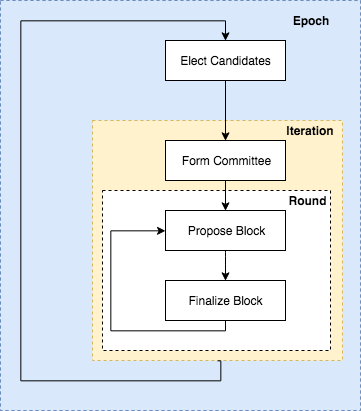
\includegraphics[width=0.5\textwidth]{Figura6}
	\label{fig:figure6}
	\caption{Randomized Delegated Proof of Stake (R-DPoS)}
\end{figure}

\subsubsection{Elezione dei candidati}
Tutti i nodi della rete IoTeX possono partecipare in questa fase votando per i candidati a far parte della commissione. Per incentivare i nodi a votare, il sistema assicura che i delegati condividano con i loro elettori le ricompense forgiate. I candidati formeranno un insieme di almeno 97 delegati; questo numero aumenterà in futuro per evitare ulteriormente il rischio di centralizzazione del consenso. Una volta selezionati i candidati, questi saranno fissati per la durata di un'epoca, che consiste di 47 iterazioni.

\subsubsection{Formazione della commissione}
In ogni iterazione, viene selezionata una commissione di 11 elementi scelti a caso mediante VRF dal pool di candidati, per la creazione dei blocchi nei successivi 11 round. L'idea è di usare l'hash del blocco dell'ultima iterazione e la chiave privata del nodo come input del VRF per produrre un output Booleano che indica se esso è stato selezionato come membro della commissione, una priorità che indica il suo livello per proporre un blocco, e una prova che indica i suoi requisiti per poter proporre il blocco in un certo round. L'uso di VRF è importante in quanto fornisce un modo non interattivo per ordinare tutti i delegati, per proporre blocchi in modo equo e in sicurezza. A tal fine, usiamo il VRF efficiente come quello utilizzato in Algorand \cite{c12}.

\subsubsection{Proposta del blocco}
In ogni round (che inizia all'incirca ogni 3 secondi), ogni nodo della commissione propone un nuovo blocco e lo trasmette alla rete, insieme con la priorità e la prova (forniti dal VRF). Solo il blocco proposto da un nodo della commissione con la priorità più alta e che non è stato già proposto nella stessa iterazione viene preso in considerazione dagli altri nodi, e viene chiamato "blocco candidato".

\subsubsection{Finalizzazione del blocco}
Nello stesso round, tutti gli altri nodi utilizzano PBFT per votare a favore o contro il blocco candidato. Se più dei 2/3 dei nodi della commissione concordano sulla validità del blocco candidato, esso viene finalizzato ed aggiunto alla blockchain da tutti gli utenti della rete. Dopo di ciò, i passi \emph{proposta del blocco} e \emph{finalizzazione del blocco} vengono nuovamente eseguiti nel round successivo; se l'iterazione corrente è terminata, sarà formata un'altra commissione a caso, prima che \emph{proposta del blocco} e \emph{finalizzazione del blocco} vengano nuovamente eseguiti.

\subsection{Creazione di checkpoint periodici per i client leggeri}
Nelle reti IoT, ci aspettiamo che molti dispositivi siano dei client leggeri, ovvero quei nodi partecipanti della blockchain che non registrano la cronologia completa delle transazioni localmente. Considerando l'overhead di archiviazione della blockchain completa, ad es. oltre 100 GB per Bitcoin \cite{c4}, molti dispositivi embedded IoT a basso costo potrebbero non avere la capacità di scaricare la blockchain completa. Tuttavia, questi client leggeri hanno ancora la capacità di verificare rapidamente la correttezza della blockchain e di interagire con essa: l'idea è inclusa nel Whitepaper originale del Bitcoin di Satoshi \cite{c21}.
Tuttavia, l'utilizzo del PoS anziché del PoW ha uno svantaggio per i client leggeri. Quando si vuole verificare la correttezza di una blockchain basata sul PoS, i client devono scaricare un elenco di chiavi pubbliche e firme per i proponenti di blocco e gli elettori, ma gli insiemi di proponenti di blocco
e gli elettori possono essere diversi per ogni singolo blocco. Quindi, quando i client leggeri tornano online dopo essere stati offline per un periodo, essi potrebbero dover scaricare un gran numero di chiavi pubbliche e firme, e quindi verificarle tutte. Per mitigare questo problema di performance, Vitalik, l'inventore di Ethereum, ha proposto di creare dei checkpoint periodici sulla blockchain, chiamate \emph{epoche} \cite{c6}, ad esempio ogni 50 blocchi. Ogni checkpoint
può essere verificato basandosi sul checkpoint precedente, in modo tale che i client leggeri possano sincronizzarsi con l'intera blockchain molto più velocemente.



\section{Token sulla rete IoTeX}
Il token digitale protetto crittograficamente nativo della rete IoTeX (IOTX) è un componente principale dell'ecosistema della rete IoTeX stessa, ed è progettato per essere utilizzato esclusivamente sulla rete. Prima del lancio della mainnet IoTeX, esso esisterà come token compatibile ERC20 sulla blockchain Ethereum, che sarà trasformato iu un token sulla mainnet IoTeX quando questa sarà avviata.

IOTX è richiesto quale "cripto-carburante" virtuale per l'utilizzo di determinate funzioni progettate sulla rete IoTeX (come l'esecuzione di transazioni e l'esecuzione di applicazioni distribuite sulla rete IoTeX), fornendo gli incentivi economici che saranno consumati per incentivare i partecipanti a contribuire a sostenere l'ecosistema sulla Rete IoTeX. Sono necessarie risorse computazionali per l'esecuzione di varie applicazioni, e per eseguire transazioni sulla rete IoTeX, così come la convalida e la verifica di ulteriori blocchi/informazioni sulla blockchain, quindi i fornitori di questi servizi/risorse hanno bisogno di incentivi economici per la fornitura di tali risorse (come ad es. avviene per il "mining" sulla rete IoTeX) per mantenere l'integrità della rete, e IOTX sarà utilizzato come unità di scambio per quantificare e pagare i costi del consumo di risorse computazionali. IOTX sarà "estraibile" per 50 anni, e le ricompense per l'attività di estrazione si ridurranno nel tempo sulla base di un modello di riduzione a gradiente lineare.

IOTX è una parte integrante e indispensabile della rete IoTeX, perché in assenza di IOTX, non ci sarebbe alcuna unità di scambio comune per pagare tali costi, rendendo così insostenibile l'ecosistema basato sulla rete IoTeX.

IOTX è un token di utilità funzionale non rimborsabile che verrà utilizzato come unità di scambio tra i partecipanti sulla rete IoTeX. L'obiettivo di introdurre IOTX è di fornire una modalità di pagamento e di accordo conveniente e sicura tra i partecipanti che interagiscono all'interno dell'ecosistema sulla rete IoTeX. IOTX non rappresenta in alcun modo una quota azionaria, partecipazione, diritto, titolo o interesse in IoTeX Foundation Ltd. (la \textbf{Fondazione}), nei suoi affiliates o in qualsiasi altra società, impresa o iniziativa, né IOTX autorizzerà i titolari di token ad alcuna promessa di commissioni, entrate, profitti o rendimenti di investimento e non sono intesi a costituire titoli a Singapore o in qualsiasi giurisdizione pertinente. IOTX può essere utilizzato solo sulla rete IoTeX, e possedere IOTX non dà diritti, espliciti o impliciti, diversi dal diritto di utilizzare IOTX come mezzo per consentire l'utilizzo e l'interazione con la rete IoTeX.

In particolare, IOTX:

\begin{enumerate}[label=(\alph*)]
    \item non è rimborsabile e non può essere scambiato con denaro contante (o il suo valore equivalente in qualsiasi altra valuta virtuale) o qualsiasi obbligo di pagamento da parte della Fondazione o qualsiasi affiliato;

    \item non rappresenta o conferisce al titolare del token alcun diritto in qualsiasi forma relativamente alla Fondazione (o a uno qualsiasi dei suoi affiliati) o alle sue entrate o attività, incluso, ma non limitato a, alcun diritto di ricevere entrate, azioni, diritto o quota su proprietà future, quota o titolo, voto, distribuzione, rimborso, liquidazione, proprietà (comprese tutte le forme di proprietà intellettuale) o altri aspetti finanziari
    o diritti legali o diritti equivalenti, o diritti di proprietà intellettuale o qualsiasi altra forma di partecipazione in relazione alla rete IoTeX, alla Fondazione, al Distributore e/o loro fornitori di servizi;

    \item non è inteso a rappresentare denaro (compreso denaro elettronico), titoli, beni, obbligazioni, strumenti di debito o qualsiasi altro tipo di strumento finanziario o investimento;

    \item non rappresenta un prestito alla Fondazione o a uno qualunque dei suoi affiliati, non è destinato a rappresentare un debito dovuto dalla Fondazione o da qualcuno dei suoi affiliati, e non esiste alcuna attesa di profitto; e

    \item non fornisce al titolare del token alcuna proprietà o altro interesse nei confronti della Fondazione o alcuno dei suoi affiliati.
\end{enumerate}


\section{Ecosistemi Basati su IoTeX}

La blockchain IoTeX supporta una varietà di ecosistemi IoT: shared economy, smart home, veicoli autonomi, supply chain, ecc. Diversi tipi di sviluppatori
sfruttano IoTeX in modi diversi. Gli sviluppatori supportati da IoTeX includono produttori di hardware IoT, sviluppatori di sistemi di controllo dei dispositivi IoT, sviluppatori di app per smart home, produttori di dispositivi per la shared economy, integratori di dati della supply chain, venditori di data crowdsourcing, sviluppatori di automobili a guida autonoma, ecc. Questa sezione descrive alcuni ecosistemi basati su IoTeX.

\subsection{Shared Economy}
Negli ultimi anni, molte aziende si sono concentrate sulla shared economy, dalla condivisione di spostamenti come Uber/Lyft/Didi, la condivisione di alloggi come Airbnb, la condivisione di biciclette come Mobike/ofo, alla condivisione di piccoli oggetti come power bank, ombrelli, ecc... Tutti forniscono
alle persone con una vita migliore, anche se alcuni di loro ricevono un danno dai loro modelli di business. Discutere questi modelli di business riguarda un altro argomento; qui ci concentriamo principalmente sulla loro architettura tecnologica. Tra tutte le economie condivise, la condivisione delle corse in auto è l'unico che non può evitare il lavoro dell'uomo, ovvero il conducente. Non è un'economia basata su IoT. Tuttavia, in futuro, quando la tecnologia delle auto a guida autonoma sarà matura e diffusa, il ride sharing sarà anch'esso basato su IoT.

Tutte le economie condivise basate IoT condividono alcune somiglianze: tutte richiedono una forma di "serratura" che può essere sbloccata da una cauzione, ed un canone di locazione. È assolutamente possibile ed anche efficiente basare l'intero processo di condivisione e restituzione utilizzando un dispositivo IoT. Nel mondo centralizzato, le economie sono basate su un cloud centralizzato. Ci sono vari inconvenienti:

\begin{enumerate}
    \item Un ingente deposito cauzionale è detenuto da una società che potrebbe non essere affidabile. Di recente ci sono stati molti casi in cui l'azienda che gestisce un servizio di bici condivise in Cina non è stata in grado di restituire i depositi ai propri utenti;

    \item Le economie condivise non sono interamente guidate dalla comunità. Molti oggetti condivisi sono di proprietà di un'azienda. Ciò ha causato uno spreco di risorse della società. Prendiam le biciclette condivise come esempio. Quando le aziende di condivisione bici chiudono l'attivita, le bici vengono eliminate.

    \item A causa della natura centralizzata, i dati dell'utente saranno archiviati e controllati da una compagnia. Ci sono rischi che il cloud o il client possano essere violati al fine di ottenere i dati degli utenti.
\end{enumerate}

IoTeX, come infrastruttura, potrebbe essere utilizzato per creare queste applicazioni senza i problemi di cui sopra e rendere le economie condivise decentralizzate e più efficienti. In concreto, un'economia condivisa basata su IoTeX offre i seguenti vantaggi:

\begin{figure}[ht]
    \centering
    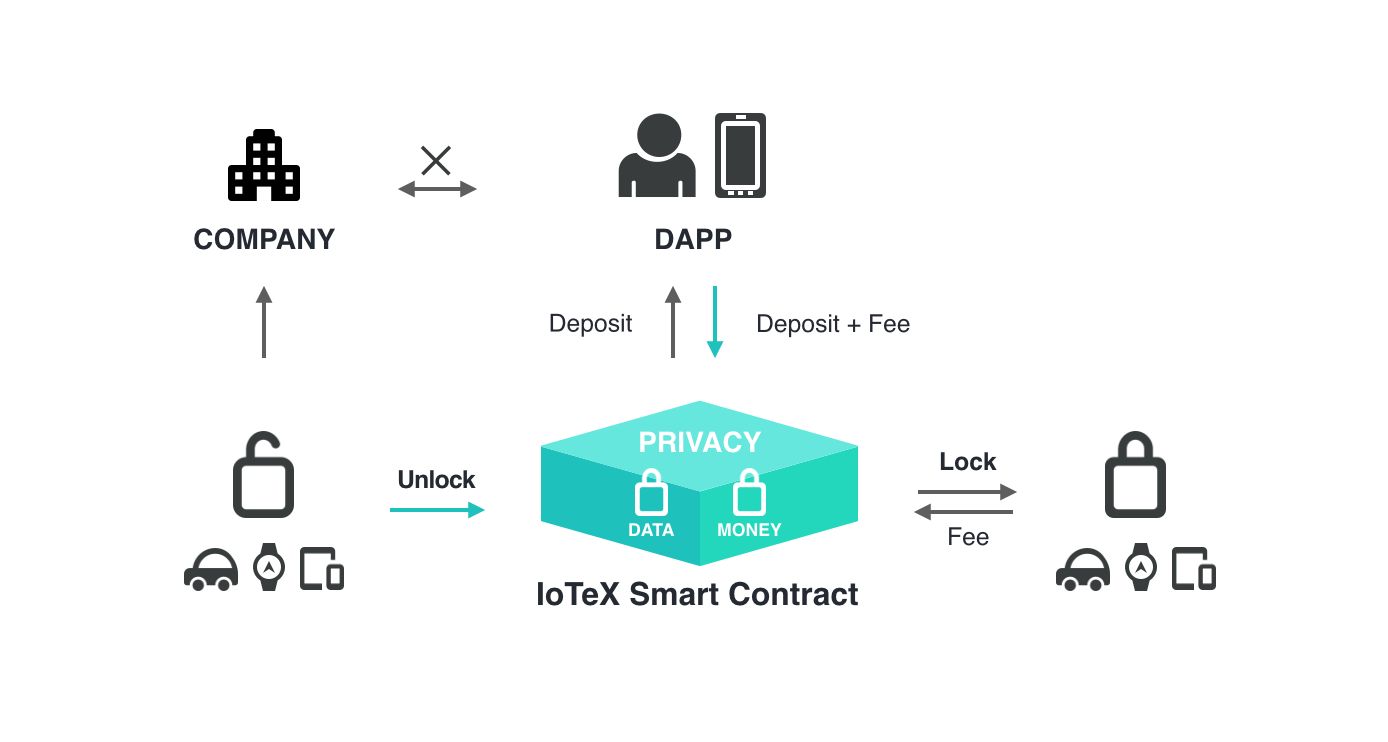
\includegraphics[width=\textwidth]{Figura7}
    \label{fig:Figura7}
    \caption{Shared Economy basata su IoTeX}
\end{figure}

\begin{enumerate}
    \item Il deposito cauzionale è interamente regolato da uno smart contract. Poiché nessuno trattiene i soldi, la restituzione del deposito è sempre garantito. Gli utenti non sono obbligati a fidarsi di una compagnia per utilizzare il servizio.

    \item Ogni oggetto condiviso realizza il suo valore e la sua missione autonomamente. Nell'ecosistema, non importa chi possiede gli oggetti in esso condivisi. Tutti possono possederle e contribuire all'ecosistema. L'economia può essere gestita dalla comunità. Di conseguenza, le aziende possono svolgere il ruolo di manutenere il blocco/serratura IoT e gestire la community. È un modello di business molto più leggero che le aziende possono  espandere velocemente e servire più persone.

    \item Ancora una volta, gli utenti non devono fidarsi dell'azienda per mantenere i propri dati. I dati sono mantenuti nella blockchain con protezione della privacy.
\end{enumerate}

La Figura \ref{fig:Figura7} descrive come funziona la shared Economy basata sulla blockchain IoTeX.

\subsection{Smart Home}

Nel mercato corrente delle smart home, molti produttori di dispositivi IoT continuano a utilizzare tecnologie obsolete per sviluppare i loro prodotti. Hanno bisogno di una grande quantità di lavoro di sviluppo sul loro cloud. Il costo di sviluppo e manutenzione è elevato, e le prestazioni sono basse a causa del viaggio andata/ritorno richiesto verso/dal cloud. Distribuendo i loro prodotti sulla blockchain IoTeX ridurrà in gran parte i costi operativi di ingegnerizzazione e cloud computing e, allo stesso tempo, aumenterà notevolmente le prestazioni dei loro dispositivi. Nel semplice esempio di una lampadina intelligente, con la tecnologia cloud, occorrono due viaggi dal comando dell'utente per cambiare lo stato di una lampadina. I produttori non sono esperti di cloud così spesso il loro servizio non è ottimale. la comunicazione tra andata e ritorno può durare da uno a tre secondi. Ciò li costringe a utilizzare i servizi cloud di grandi aziende IT. Ci sono due aspetti negativi dell'utilizzo di questi servizi cloud:

\begin{enumerate}
    \item I produttori non possono controllare completamente la disponibilità dei servizi cloud.

    \item Hanno bisogno di pagare continuamente per il servizio cloud a fronte di un incasso una tantum per la vendita dei loro dispositivi IoT.

    \item Ci sono rischi di hacking del loro cloud, in caso di hacking lato client o intranet i dati degli utenti verrebbero trafugato oppure si creerebbero problemi di sicurezza domestica.
\end{enumerate}

Al contrario, la blockchain IoTeX gestisce i dispositivi localmente e interagisce con la blockchain pubblica su internet quando necessario. La blockchain pubblica è gestita dalla comunità. Non ci sono costi di manutenzione per i produttori di IoT. La blockchain di IoTeX dispone di protezione della privacy il che può impedire la perdita di dati sensibili o che l'unità di controllo venga hackerata anche se la rete intranet non è sicura.

\begin{figure}
    \centering
    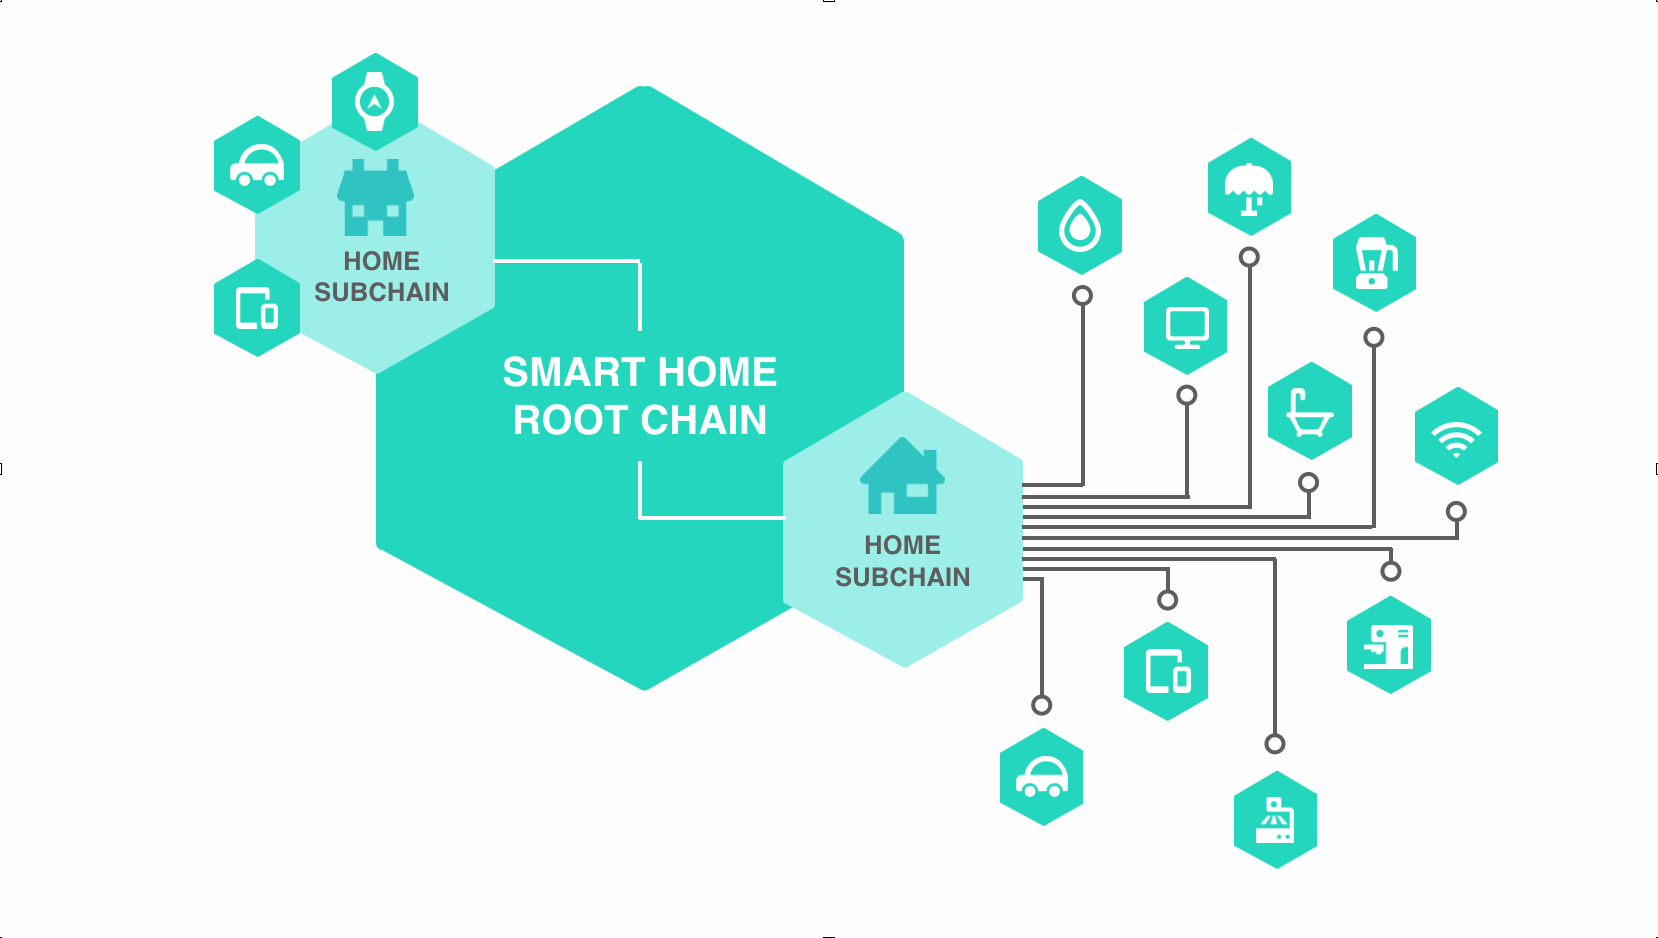
\includegraphics[width=\textwidth]{Figura8}
    \label{fig:Figura8}
    \caption{Smart Home basata su IoTeX}
\end{figure}

Oltre a consentire ai produttori di IoT di implementare i loro dispositivi IoT sulla blockchain IoTeX, IoTeX collaborerà con i produttori di chip IoT per sviluppare chip abilitati all'uso della blockchain IoTeX per accelerare il ciclo di progettazione e produzione di dispositivi IoT. I produttorio di dispositivi IoT semplicemente integreranno il chip per fare in modo che i loro dispositivi siano supportati dlla blockchain IoTeX.


\subsection{Gestione delle identità}
Il mondo in crescita dell'IoT ha avuto un impatto su come la gestione delle identità e degli accessi (\emph{Identity and Access Management} - IAM)
deve funzionare. In termini di identità delle cose, lo IAM deve essere in grado di gestire il sistema utente-dispositivo, dispositivo-dispositivo, e/o dispositivo-servizio. Un modo semplice per la gestione dell'identità è quello di considerare la blockchain IoTeX come un sistema PKI decentralizzato
(grazie alla sua immutabilità) in cui a ciascuna entità viene rilasciata un'identità crittografica sotto forma di certifcato TLS e la chiave privata corrispondente. Questo certificato, che tendenzialmente è di breve durata, viene firmato dal certificato di lunga durata integrato nel dispositivo, e poi pubblicato sulla blockchain IoTeX (rootchain o subchain). I nodi ed altre entità possono accedere e fidarsi del certificato di breve durata ancorato alla
blockchain, e i dispositivi possono quindi autenticarsi quando arrivano online, garantendo sicurezza di comunicazione tra altri dispositivi, servizi e utenti e dimostrare la loro integrità.

Inoltre, è possibile organizzare gerarchicamente i certificati longevi integrati nei dispositivi, come per la PKI convenzionale, in cui i dispositivi genitore possono firmare i certificati dei figli. Grazie alla gerarchia, diventa possibile la revoca e la rotazione dei certificati. Ad esempio, se un dispositivo viene compromesso, il suo dispositivo genitore o anche il dispositivo nonno potrebbero firmare un comando di revoca e inviarlo alla blockchain dove quest'ultimo invalida il certificato del dispositivo.

\section{Lavori di ricerca futuri}
Alcune direzioni di ricerca già in corso ed altre future per migliorare IoTeX sono indicate di seguito.

\paragraph{Potenza di calcolo per il mantenimento della privacy}
Ci sono diverse aree in questa direzione che stiamo esplorando attivamente:

\begin{itemize}
    \item Come mantenere gli stati confidenziali sulla blockchain, in modo che possano essere utilizzati per il calcolo da un certo gruppo di nodi;

\item Smart contract in grado di preservare la privacy, dove lo smart contract può essere eseguito nonostante la sua business logic sia protetta dalla crittografia. Mentre la crittografia completamente omofobica \cite{c26} e gli schemi di offuscamento indistinguibile \cite{c11} rappresentano il "Santo Graal" solo in teoria, proposte pratiche come Hawk \cite{c17} sono promettenti per il prossimo futuro;

\item Ulteriore risuzione dei requisiti computazionali e dello spazio di archiviazione necessari per le tecniche di preservazione della privacy che IoTeX sta attualmente utilizzando;

\item La versione quantum-safe delle tecniche di conservazione della privacy che IoTeX utilizza attualmente, ad esempio una ring signature quantum-safe.
\end{itemize}


\paragraph{Pruning e Trasferimento degli Stati}
Stiamo valutando diversi modi per sfoltire in maniera sicura gli stati memorizzati nelle subchain, per ridurre l'ingombro di storage dal momento che molti dispositivi IoT dispongono di spazio di archiviazione limitato. La compressione di blocchi e transazioni risulta sicuramente una soluzione comoda. Inoltre, anche trasferire gli stati da una subchain alla rootchain (dal momento che quest'ultima è più dotata in termini di spazio di archiviazione) in maniera efficiente e con salvaguardia della privacy rappresenta un argomento insteressante da indagare.

\paragraph{Governance auto-adattativa}
Mentre la blockchain IoTeX offre incentivi per mantenere il consenso sui suoi registri, per il momento non dispone di un meccanismo in grado di auto-modificare le regole che governano il suo protocollo. Per affrontare ciò, abbiamo in programma di condurre ricerche su governance e auto-modifica.

\paragraph{Blockchain con struttura ad albero}
L'attuale blockchain IoTeX ha due livelli e, naturalmente, potrebbe essere estesa a un albero di blockchain sfruttando tecniche simili a quelle utilizzate in Plasma e Cosmo. Il piano è quello di valutare queste proposte e migliorare l'attuale progetto di IoTeX, ed alla fine supportare strutture gerarchiche più complesse.

\section{Conclusioni}
In questo Whitepaper, abbiamo introdotto IoTeX, una blockchain scalabile, privata, ed estensibile, dedicata all'Internet of Things, con la sua architettura e le sue tecnologie di base, che includono:

1. Blockchain in blockchain, per massimizzare scalabilità e privacy, 2. privacy totale su blockchain basata su codice di pagamento inoltrabile, ring signature a dimensione costante e senza configurazione trusted, e implementazione iniziale di bulletproofs, 3. consenso rapido con finalità istantanea basata su VRF e PoS per volumi di transazioni elevati e finalità istantanea e 4. architetture di sistema basate su IoTeX flessibili e leggere.

\section{Ringraziamenti}
Vogliamo esprimere la nostra gratitudine ai nostri mentori e consulenti e alle molte persone nelle comunità dell'IoT, della crittografia e delle criptovalute per i loro feedback iniziali e i suggerimenti costruttivi.

\pagebreak

\begin{otherlanguage}{english}
	\bibliographystyle{plain}
	\bibliography{bibliography}
\end{otherlanguage}



\end{document}